% todo: refactor S(G) to gamma


\documentclass[a4paper,12pt]{report}
\usepackage[T1]{fontenc}
\usepackage{lmodern}
\usepackage{amssymb,amsmath}
\usepackage{ifxetex,ifluatex}
\usepackage{fixltx2e} % provides \textsubscript
\usepackage[english, ngerman]{babel}

\usepackage{lmodern} \normalfont %to load T1lmr.fd 
\DeclareFontShape{T1}{lmr}{bx}{sc} { <-> ssub * cmr/bx/sc }{}


% use upquote if available, for straight quotes in verbatim environments
\IfFileExists{upquote.sty}{\usepackage{upquote}}{}
\ifnum 0\ifxetex 1\fi\ifluatex 1\fi=0 % if pdftex
  \usepackage[utf8x]{inputenc}
\else % if luatex or xelatex
  \usepackage{fontspec}
  \ifxetex
    \usepackage{xltxtra,xunicode}
  \fi
  \defaultfontfeatures{Mapping=tex-text,Scale=MatchLowercase}
  \newcommand{\euro}{€}
\fi
% use microtype if available
\IfFileExists{microtype.sty}{\usepackage{microtype}}{}
\ifxetex
  \usepackage[setpagesize=false, % page size defined by xetex
              unicode=false, % unicode breaks when used with xetex
              xetex,
              linkcolor=black
              ]{hyperref}
\else
  \usepackage[unicode=true,linkcolor=black]{hyperref}
              
\fi
\hypersetup{breaklinks=true,
            pdfauthor={},
            pdftitle={},
            colorlinks=true,
            urlcolor=blue,
            linkcolor=magenta,
            pdfborder={0 0 0}}
\urlstyle{same}  % don't use monospace font for urls
\setlength{\parindent}{0pt}
\setlength{\parskip}{6pt plus 2pt minus 1pt}
\setlength{\emergencystretch}{3em}  % prevent overfull lines
\setcounter{secnumdepth}{0}

% Treeview
\usepackage{tikz}
\usepackage{tikz-qtree}

\hypersetup{linkcolor = black}

% Graphviz
\usepackage{graphvizzz}

% Source Code so found here: http://en.wikibooks.org/wiki/LaTeX/Source_Code_Listings
\usepackage{color}
\usepackage{listings}
\lstset{ %
basicstyle=\footnotesize,       % the size of the fonts that are used for the code
numbers=left,                   % where to put the line-numbers
numberstyle=\footnotesize,      % the size of the fonts that are used for the line-numbers
stepnumber=1,                   % the step between two line-numbers. If it is 1 each line will be numbered
numbersep=5pt,                  % how far the line-numbers are from the code
backgroundcolor=\color{white},  % choose the background color. You must add \usepackage{color}
showspaces=false,               % show spaces adding particular underscores
showstringspaces=false,         % underline spaces within strings
showtabs=false,                 % show tabs within strings adding particular underscores
frame=single,           % adds a frame around the code
tabsize=2,          % sets default tabsize to 2 spaces
captionpos=b,           % sets the caption-position to bottom
breaklines=true,        % sets automatic line breaking
breakatwhitespace=false,    % sets if automatic breaks should only happen at whitespace
escapeinside={\%*}{*)}          % if you want to add a comment within your code
}

% Definitionen
\usepackage{amsthm}

% Algorithmen
\usepackage{algpseudocode}
\usepackage{algorithm}

%todo 
\usepackage[colorinlistoftodos,prependcaption,textsize=tiny]{todonotes}

\usepackage{xargs}                      % Use more than one optional parameter in a new commands


\usepackage{url}

\linespread{1.1}



\setcounter{secnumdepth}{3}
\setcounter{tocdepth}{1}



% TODO: add improve and question
\newcommandx{\IMPROVE}[2][1=]{\todo[linecolor=none,backgroundcolor=orange!25,bordercolor=none,#1]{\textbf{IMPROVE: }#2}}
\newcommandx{\QUESTION}[2][1=]{\todo[linecolor=none,backgroundcolor=blue!15,bordercolor=none,#1]{\textbf{QUESTION: }#2}}
\newcommandx{\TODO}[2][1=]{\todo[linecolor=none,backgroundcolor=gray!25,bordercolor=none,#1]{\textbf{TODO: }#2}}

\def\signed #1{{\leavevmode\unskip\nobreak\hfil\penalty50\hskip2em
  \hbox{}\nobreak\hfil(#1)%
  \parfillskip=0pt \finalhyphendemerits=0 \endgraf}}

\newsavebox\mybox
\newenvironment{aquote}[1]
  {\savebox\mybox{#1}\begin{quote}}
  {\signed{\usebox\mybox}\end{quote}}


\newtheorem{mydef}{Definition}
\renewcommand*\contentsname{Inhaltsverzeichnis}

\author{Denis Erfurt}
\date{\now}
\title{Ein dezentrales Transitionssystem zur manipulation von Wörtern einer regulären Sprache}


\begin{document}

\begin{titlepage}
\hspace{0cm}
\vspace{-2cm}
 
\begin{flushright}

\includegraphics[width=3.2 cm]{bilder/husiegel.pdf}
\end{flushright}
 
 
\begin{center}
  \vspace{0.5 cm}
  \LARGE{\bf Ein dezentrales Transitionssystem zur Manipulation von geteilten Wörtern einer regulären Sprache} \\ % Hier fuegen Sie den Titel Ihrer Arbeit ein.
  \vspace{1 cm}
  \LARGE  Bachelorarbeit \\ % Geben Sie anstelle der Punkte an, ob es sich um eine
                % Diplomarbeit, eine Masterarbeit oder eine Bachelorarbeit handelt.
  \vspace{1cm}
  \Large zur Erlangung des akademischen Grades \\
  Bachelor of Science (B. Sc.) \\ % Bitte tragen Sie hier anstelle der Punkte ein:
         % Diplominformatiker(in),
         % Bachelor of Arts (B. A.),
         % Bachelor of Science (B. Sc.),
         % Master of Education (M. Ed.) oder
         % Master of Science (M. Sc.).
  \vspace{1.0cm}
  {\large
    \bf{
      \scshape
      Humboldt-Universit\"at zu Berlin \\
      Institut f\"ur Informatik\\
    }
  } 
  % \normalfont
\end{center}
\vspace{1.0 cm}
{\large
  \begin{tabular}{llll}
    eingereicht von:    & Denis Erfurt && \\ % Bitte Vor- und Nachnamen anstelle der Punkte eintragen.
    geboren am:         & 02.04.1988 && \\
    in:                 & Novosibirsk && \\
    &&&\\
    Gutachter(innen): & Prof. Dr. Klaus Reinhardt && \\
              & Prof. Dr. Jens-Peter Redlich && \\% Bitte Namen der Gutachter(innen) anstelle der Punkte eintragen
    &&&\\
    eingereicht am:     & \dots\dots \hspace{3cm} verteidigt am: & & \dots\dots \\ % Bitte lassen Sie
                                    % diese beiden Felder leer.
                                    % Loeschen Sie ggf. das letzte Feld, wenn
                                    % Sie Ihre Arbeit laut Pruefungsordnung nicht
                                    % verteidigen muessen.
  \end{tabular}
}
 
\end{titlepage}

\thispagestyle{empty}
 
%%%%%%%%%%%%%%%%%%%%%%%%%%%%%%%%%%%%%%%%%%%%%%%%%%%%%%%%%%%%%%%%%%%%%%%%%%%%%%%%%%%%%%%%%%%%%%%%%%%%
%% Selbststaendigkeitserklaerung
%%%%%%%%%%%%%%%%%%%%%%%%%%%%%%%%%%%%%%%%%%%%%%%%%%%%%%%%%%%%%%%%%%%%%%%%%%%%%%%%%%%%%%%%%%%%%%%%%%%%
 
{\parindent 0cm
%%%%%%%%%%%%%%%%%%%%%%%%%%deutsche Version%%%%%%%%%%%%%%%%%%%%%%%%%%%%%%
   
  \subsection*{Selbst\"andigkeitserkl\"arung}
  Ich erkl\"are hiermit, dass ich die vorliegende Arbeit selbst\"andig verfasst 
  und nur unter Verwendung der angegebenen Quellen und Hilfsmittel angefertigt habe. 
  Weiterhin erkl\"are ich, eine Bachelorarbeit in diesem Studiengebiet erstmalig einzureichen.\\
%statt der Punkte Diplom, Master oder Bachelor angeben
  \vspace{3\baselineskip}
   
  Berlin, den \today \hspace{0.25\linewidth}\parbox{0.3\linewidth}{\dotfill}
 
%%%%%%%%%%%%%%%%%%%%%%%%%%englische Version%%%%%%%%%%%%%%%%%%%%%%%%%%%%%%%%%%%%%%%%%%%%%%%%%%%%%%%%%
\selectlanguage{english}
\subsection*{Statement of authorship}
I declare that I completed this thesis on my own and that information which has been 
directly or indirectly taken from other sources has been noted as such. Neither this 
nor a similar work has been presented to an examination committee.
 
  \vspace{3\baselineskip}
   
  Berlin, \today \hspace{0.25\linewidth}\parbox{0.3\linewidth}{\dotfill}
}



\section*{Abstract}
% überblick
% problembeschreibung, literaturüberblick, related work, 

% Es geht um Akteure, Besitz, Bewertung

% sowie die Bewertung konkurierender Beitragskandidaten, deren Komposition 
% 
% sowie der repräsentation des Inhaltes aus einer Kandidatenmenge. 
% 
% sowie nach den \textbf{Bewertungen} der einzelnen Beiträge durch die Besitzer, deren Komposition als Gesamtergebnis den eigendlichen Inhalt biltet.
% 
% sowie der eigendlichen Form des Inhaltes, welches eine Komposition einzelner Beiträge ist



% Eine besitzbare Einheit kann als eine bestimmte Struktur von Teilen angesehen werden. Die Teile sind wiederum besitzbare Einheiten, deren Besitz vorerst unabhängig vom Besitz des Ganzen ist. Intuitiev sollte der Besitz des Ganzen proportional zu der komposition der Teile sein. Dabei entstehen folgende Fragem:
% - wie berechnet sich die gewichtung eines Teiles.

% Intuitiev sollte der initialle Besitzer eines Inhalts sein Schöpfer sein. Dieser kann sein Besitz bei einer einigung an dritte abgeben, oder der Allgemeinheit überlassen. Bei einem Kollaborativ entstandenem Inhalt, bewerten die Besitzer die Beiträge


% Problem: der Verwaltung( Manipulation ) und der besitzallokation

Im Internet werden zunehmend Inhalte kollaborativ erzeugt. 
Dabei entsteht ein Inhalt durch Beiträge einzelner Akteure, die räumlich und zeitlich getrennt sein können.
Zentral ist dabei die Frage wie der Konsens über einen Inhalt auf eine dezentrale Weise gebildet werden kann.
In dieser Arbeit untersuchen wir den Prozess der verteilten Zusammenarbeit für Inhalte die als Wörter einer regulären Sprache beschrieben werden können. Dafür wird ein Modell mit einer Implementation einer Blockchain-Technologie vorgestellt: Ein öffentliches Transitionssysthem mit dezentral validierter Ausführung. 
Ebenfalls wird eine Grammatik-Erweiterung mit einer Konsens-Funktion für eine beliebige reguläre Grammatik beschrieben. Die Wörter der erweiterten Grammatik beinhalten Informationen über die Besitzallokation der Akteure, alternative Beiträge und deren Bewertung. 
Die Konsens-Funktion überführt unter Berücksichtigung der Bewertungen ein Wort der erweiterten Grammatik in ein Wort der ursprünglichen Grammatik.


% Outline - kurze konkrete zusammenfassung was kommt



% 


\newpage
\tableofcontents


%%%%%%%%%%%%%%%%%%%%%%%%%%%%%%%%%%%%%%%%%%%%%%%%%%%%%%%%%%%%%%%%%
%%%%%%%%%%%%%%%%%%%%%%%%%%%%%%%%%%%%%%%%%%%%%%%%%      EINLEITUNG
%%%%%%%%%%%%%%%%%%%%%%%%%%%%%%%%%%%%%%%%%%%%%%%%%%%%%%%%%%%%%%%%%


\newpage

\chapter{Einleitung}

Nehmen wir z.B. an, es gäbe eine Webseite, die sich im Besitz von Akteuren befindet. Alle Akteure wollen gerecht, also proportional zu ihrem Besitz, über die Inhalte der Webseite entscheiden können, sowie ihre Entscheidungsgewalt in bestimmten Bereichen an andere vertrauenswürdige Akteure delegieren können. Dieses gilt für die medialen Inhalte, die Programmierung, die Architektur, die Wertflüsse wie ein geteiltes Budget oder eine Einkommensverteilung, sowie nicht automatisierbare Prozesse, wie das Validieren neuer Beiträge. Das eigentliche Ergebnis wird anhand von einer Mehrheit der Besitzer bestimmt.

Wikipedia folgt einem streng hierarchischem Modell, in welchem Vertrauenspersonen die Inhalte der Benutzer filtern. Die Verantwortung liegt bei der Organisation.
Effizienter sind jedoch selbstregulierende Systeme, bei denen die Benutzer die Inhalte der Anderen bewerten. Beispiele wären die auf Voting und Reputation basierenden Plattformen Reddit und StackOverflow.
Ein weiteres Beispiel für die Bewertung von Inhalten ist das Konzept 
Liquid Democracy\cite{Lindenberg2010}, ein Vorschlag der Piratenpartei für eine moderne politische Konsensbildung.
Ein solches Prinzip könnte man auf das Verwalten aller digital geteilter Inhalte verallgemeinern.

Jedoch eignen sich diese Konzepte nur bedingt um damit geteiltes Eigentum wie z.B. eine Webseite zu modellieren, da Abstimmungen auf eine informale Weise vorgenommen werden. Es fehlt einer formalen Syntax, welche die Implikationen einer potentiellen Entscheidung vor der Wahl durch Simulation klarer zeigt, sowie nach der Wahl automatisch ausführt.
Außerdem bedarf es bei den Ansätzen eines zentralisierten Servers, welcher als Angriffspunkt die Glaubwürdigkeit des Prozesses gefährdet, da die Akteure auf die Korrektheit des Servers vertrauen müssen. 

Das 2009 eingeführte Konzept des Bitcoins und der Blockchain\cite{Nakamoto2008} bietet eine Alternative zur zentralen Server-Architektur. Dieses beschreibt ein Protokoll in einem Netzwerk, welches Inhalte aus einem gebildeten Konsens bereitstellt. Es besitzt eine einfache, nicht turing vollständige Skriptsprache, sowie durch ein asymmetrisches Kryptosystem, Rechte und Rollen. Neue Inhalte werden nach einer Validierung ebenfalls in den Konsens aufgenommen. Die einfachste Interpretation von Bitcoin ist die eines Werteträgers, wobei die Beschränkung der Skriptsprache wenig Spielraum für weitere Interpretationen lässt.
Allgemeiner ist das auf dem Bitcoin-Protokoll aufbauende Ethereum\cite{Wood2014} , welches eine turing vollständige Skriptsprache besitzt.
Es entsteht eine Vielzahl von neuen Anwendungsmöglichkeiten: verbindliche, autonome Verträge zwischen mehreren Parteien, Dezentrale-Autonome-Organisationen (DAO) oder profitorientierte Kooperationen (DAC), die allesamt Werte- und Informationsflüsse ermöglichen.
Ein Beispiel einer solchen DAO ist das namecoin\footnote{http://namecoin.info/} Konzept, welches als Alternative zur ICANN\footnote{Internet Corporation for Assigned Names and Numbers} Organisation die TLD ``.bit'' verwaltet und in naher Zukunft die ICANN ablösen könnte.\cite{Corporation2014} Die Regeln unter denen DACs und DAOs funktionieren, wie das Bewilligen einer neuen TLD, werden auf der Ethereum Plattform programmiert.
Die Einigung der Akteure auf ein Programmstand geschieht noch durch eine zentrale Vertrauensinstanz, z.b. bestimmten Schlüsselpersonen.


\section*{Leistung und Struktur der Arbeit}
In dieser Arbeit versuchen wir die Frage zu beantworten, wie eine Menge von Akteuren auf eine dezentrale Weise einen Konsens über ein Wort einer regulären Sprache bilden kann.
Die Arbeit besteht im wesentlichen aus drei Teilen: Sie fasst notwendige Theoretische Grundlagen zusammen. Auf diese Aufbauend wird ein Modell für eine Selbst-Modifikation-Schicht einer DAO ausgearbeitet und auf DAOs mit regulären Grammatiken angewandt. Schließlich wird das ausgearbeitete Modell Implementiert.

Die weitere Arbeit ist wie folgt aufgebaut: In Kapitel \ref{theo} werden Theoretische Konzepte beschrieben auf denen diese Arbeit aufbaut. Ebenfalls wird eine ausführliche Definition einer Dezentralen-Autonomen-Organisation gegeben, wie sie zum Zeitpunkt der Arbeit vorliegt. Darauf aufbauend wird das Problem der Selbst-Modifikation erläutert und in Kapitel \ref{selfMod} eine Definition sowie eine Anwendung auf die regulären Sprachen erarbeitet. In Kapitel \ref{implementation} wird eine Implementation der Anwendung vorgestellt. Schließlich wird in Kapitel \ref{ausblick} eine Zusammenfassung der Ergebnisse, sowie ein Ausblick gegeben. 


\chapter{Theoretische Grundlagen}
\label{theo}

%%%%%%%%%%%%%%%%%%%%%%%%%%%%%%%%%%%%%%%%%%%%%%%%%%%%%%%%%%%%%%%%%
%%%%%%%%%%%%%%%%%%%%%%%%%%%%%%%%%%%%%%%%%%%%%%      VERIFIZIERUNG 
%%%%%%%%%%%%%%%%%%%%%%%%%%%%%%%%%%%%%%%%%%%%%%%%%%%%%%%%%%%%%%%%%

Dieser Kapitel fasst theoretische Grundlangen zusammen, auf denen die Nachfolgenden Kapitel aufbauen. In Abschnit \ref{regGram} werden die Regulären Grammatiken vorgestellt sowie die Kontextfreien Grammatiken in Abschnit \ref{cfGram}. In Abschnit \ref{trie} wird die Trie Datenstruktur betrachtet. In Abschnit \ref{transSys} wird das initiale Transitionssysthem eingeführt. In Abschnit \ref{crypt} wird die asymetrische Verschlüsselung betrachtet.

\section{Reguläre Grammatiken}
\label{regGram}
Eine reguläre Grammatik definiert nach Noam Chomsky ist ein vier Tupel 
$G = (N,T,S,P)$ bestehend aus 

\begin{enumerate}
\item $N$ - einer Menge nichtterminaler Symbole 
\item $T$ - einer Menge terminaler Symbole, mit $T\cap N = \emptyset$
\item $S\in N$ - einem Startsymbol
\item $P \subseteq N\times \{\epsilon\}\cup T \cup TN$ - einer Menge von Produktionen oder auch Produktionsregeln
\end{enumerate}

Sei weiter $\Sigma := N \cup T$ das Alphabet der Grammatik.

Eine Produktion $(R,r)\in P$ kann auch als $R\rightarrow r$ geschrieben werden.
Sie sagt aus, dass das Nichtterminal R in einem Schritt überführt werden kann zum Teilwort r:

\begin{eqnarray}
  \alpha R \rightarrow \alpha r
\end{eqnarray}

Sind hierfür n Schritte notwendig, schreibt man $R \rightarrow^n r$. Um auszudrücken, dass $r$ generell aus $R$ ableitbar ist, kann man sich der reflexiv-transitiven Hülle der Produktionsregeln bedienen: $R \rightarrow ^* r$.

Die Sprache, die von der regulären Grammatik erzeugt wird, ist die Menge aller Wörter, die vom Startsymbol ableitbar sind: 
\begin{eqnarray}
  L(G) := \{w | S \rightarrow^* w \land w\in T^* \} 
\end{eqnarray}
Existiert eine reguläre Grammatik, die eine Sprache erzeugt, so heißt die Sprache ebenfalls regulär.

Die Klasse der regulären Sprachen heißt $REG$.

Ein Beispiel für eine reguläre Grammatik mit der dazugehörigen Sprache ist: 

\begin{center}
 $
\begin{array}{rcl}
  G_{abc} &=& (N,T,S,P) \\
  N &=& \{ S, A, B, C \} \\
  T &=& \{ a, b, c \} \\
  P &=& \{ \\ 
  &&  S \rightarrow a A,
    S \rightarrow b B,
    S \rightarrow c C,
    S \rightarrow \varepsilon,\\
  &&  A \rightarrow a A,
    A \rightarrow b B,
    A \rightarrow c C,
    A \rightarrow \varepsilon,\\
  &&  B \rightarrow b B,
    B \rightarrow c C,
    B \rightarrow \varepsilon, \\
  &&  C \rightarrow c C,
    C \rightarrow \varepsilon,\\
  &&\}
\end{array}
\label{regGramEx}
$ 
\end{center}

\begin{eqnarray}
  L(G) = \{ a^xb^yc^z | x,y,z\in \mathbb{N} \} 
\end{eqnarray}



\section{Kontextfreie Grammatiken}
\label{cfGram}

Kontextfreie Sprachen unterscheiden sich nur in den Produktionsregeln von den regulären. Anders als bei regulären, wird für die rechte Seite einer Produktionsregel keine Einschränkung gemacht: $P \subseteq N\times (N\cup T)^*$

% \subsection*{Greibach-Normalform}
% Da eine reguläre Grammatik ein Spezalfall einer Kontextfreien Grammatik ist und jede Kontextfreie Grammatik in der Greibach-Normalform darstellbar ist ist jede reguläre Grammatik ebenfalls in der Greibach-Normalform darstellbar.
% 
% Warum muss die reguläre Grammatik in der Greibach-Normalform sein?
% Durch die Grammatikerweiterung werden die Regeln der Regulären Grammatik mit Optionsmengen erweitert. Gibt es eine Regel $A->B$, kommt es du einer mehrdeutung der Ableitung da eine Optionsmenge bei $A$ und $B$ erzeugt wird.


\subsection*{Wortteil}

Sei $G=(S,N,T,P)$ eine Grammatik und $w\in L(G)$, dann definieren wir ein Wortteil: 

\begin{eqnarray}
  w_{i..j} := 
  \begin{cases}
    (t_k)_{i\leq k \leq j}\text{ mit }t_k\in T &:\ i\leq j \\
    \varepsilon &:\ i>j
  \end{cases}
\end{eqnarray}

\section{Trie}
\label{trie}

Ein Trie oder Prefixbaum ist eine Baum-Datenstruktur, die es erlaubt eine Menge von Worten über einem Alphabet effizient zu Speichern. Dabei werden gemeinsame Präfixe von wörtern in Knoten zusammengefasst.
Eine Trie verwandte Datenstruktur, die Patricia-Trie reduziert den Speicherverbrauch indem sie alle Knoten mit nur einem Nachfolger zu einem Knoten zusammenfasst.
Alle im Trie und Patricia-Trie gespeicherten Wörter können durch ein Tiefenscan wiederhergestellt werden. \cite{Morrison1968}
Ein Beispiel eines Patricia-Trie für die Menge $\{ aaaaa, aac, aacc, aaccc, aabbb, aabb \}$ zeigt die Abbildung \ref{trieImg}.

\begin{figure}[ht]
    \centering
    \Tree [.aa aaa c [.c c cc ] [.b bb b ] ]
    \caption{Beispiel einer Patricia-Trie Datenstruktur}
    \label{trieImg}
\end{figure}

\section{Transitionsystem}
\label{transSys}

Ein initialisiertes Transitionssystem ($T$) \cite{Glausch} gibt einen formalismus vor um ein zustandbasiertes System zu beschreiben. Die Beschreibung zerteilt sich in die des Zustandraumes, beschrieben durch eine Menge $M$, die der Dynamik, beschrieben durch eine Übergangsfunktion $\tau: M \rightarrow M$ und einer Anfangszustandsmenge $I\subset M$.

\begin{eqnarray}
   T = (M,I,\tau)
\end{eqnarray}

\subsection*{Ablauf}
Eine Folge $(s_n)_{n\in\mathbb{N}}$ mit $s_n\in M$ ist ein Ablauf von T, wenn gilt:

\begin{eqnarray}
   s_0 \in I \\
   s_{i+1} = \tau(s_i) 
\end{eqnarray}

% section  (end)

\section{asymetrische Verschlüsselung}
\label{crypt}

% \begin{figure}[ht]
%     \centering
%     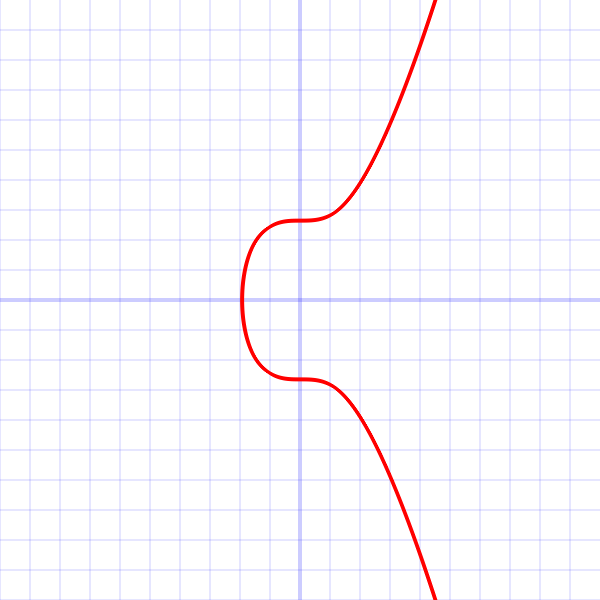
\includegraphics[width=0.50\textwidth]{bilder/Secp256k1.png}
%     \caption{ECDSA - secp256k1 Kurve https://en.bitcoin.it/wiki/File:Secp256k1.png 25.02.2015}
% \end{figure}

% \subsection*{asymetrische Verschlüsselung}
Bei einem asymmetrischem Verschlüsselungsverfahren generiert der Benutzer ein Schlüsselpaar bestehend aus einem privatem und einem öffentlichem Schlüssel. Der öffentliche Schlüssel wird aus dem Privaten erzeugt und veröffentlicht. Wir werden im Folgenden den öffentlichen Schlüssel ebenfalls Adresse nennen. Die identifiziert einen Akteur.

Für die Signierung und Verifizierung von Nachrichten wird ECDSA mit der secp256k1 Kurve verwendet. ECDSA ist eine DSA Verfahren basierend auf Eliptic Curve Kryptografie. ECDSA bietet viele Vorteile zu alternativen Verfahren wie RSA oder DH.\cite{Pouillard2014}
% 
% \subsection*{Signierung}
% 
% Eine Aktion( oder auch Nachricht (msg) genannt) eines Akteurs kann mit dem privatem schlüssel signiert werden.
% \[ signMsg: priv \times msg \rightarrow sign \] 
% Mithilfe einer weiteren Funktion kann nun durch die öffentliche Addresse des Akteurs, der nachricht und deren Signatur verifiziert werden, ob die Nachricht auch tatsächlich vom angegebenem Akteur ausgelöst wurde.
% \[ verifyMsg: msg \times sign \times addr \rightarrow \{ True, False \} \] 
% Dadurch besteht nun eine Aktion eines Akteurs aus der nachricht, seiner Addresse sowie der signatur der nachricht.
% 
% \[ (msg, sign, addr) \]
% 
\chapter{Decentralized Autonomous Organization (DAO)}
\label{daoEinf}
In diesem Kapitel wird der Begriff der Decentralized Autonomous Organization Ausführlich betrachtet und diskutiert. Dabei folgt nach einer Einführung in Kapitel \ref{blockchain} die Betrachtung der dezentralisierenden Technologie: der Blockchain. In Kapitel \ref{interaction} wird die Interaktion mit einer DAO betrachtet.

Eine DAO ist ein relativ neues Konzept, welches durch das populärwerden von Technologien wie Bitcoin und Ethereum erstmals aufgetaucht ist. Die Fachwelt ist sich noch über die genaue Definition und die Abgrenzung zu verwanten Konzepten größtenteils uneinig.

\begin{aquote}{Vitalik Buterin - Ethereum Founder - 06.05.2014\footnotemark}
 One of the most popular topics in the digital consensus space [...] is the concept of decentralized autonomous entities. [...] However, one of the hidden problems lurking beneath the space is a rather blatant one: no one even knows what all of these invididual terms mean. 
\end{aquote}
\footnotetext{https://blog.ethereum.org/2014/05/06/daos-dacs-das-and-more-an-incomplete-terminology-guide/ }

Zwar existieren Versuche ``Decentralized Applications'' (DAs,Dapps) wie BitTorrent oder den ``Decentralized Autonomous Corporations'' (DACs) von dem der DAOs Abzugrenzen, jedoch gibt es hier keine Garantie auf Persistenz der Terminologie sowie ihrer Definitionen, deshalb werden im Folgenden die Begriffe DA, Dapp, DAC, DAO synonym verwendet.

Intuitiv kann eine DAO als eine Gesellschaft verstanden werden, die ohne menschliche Einwirkung existiert und agiert. Sie kann ebenfalls als eine erweiterung des Open-Source Konzeptes betrachtet werden. Dabei ist nicht nur der Programmcode öffentlich, sondern auch ihre internen Berechnungen sowie wesentliche Teile ihrer Interaktionen. Diese sind durch einen gemeinsamen Konsens von der Erzeugung bis zum aktuellen Zustand determiniert und nachvollziehbar. Dieser Konsens wird auf eine dezentrale Weise gebildet, um zu verhindern, dass eine zentrale Instanz den Konsens manipuliert sowie um Robustheit und Beständigkeit zu sichern.

In ihren Aktionen kann die DAO interne, deterministische Berechnungen anstellen, mit anderen DAOs kommunizieren und so auf Services zugreifen oder nicht selbst ausführbare Aufgaben, wie beispielsweise das Erweitern und Verbessern des Programmcodes, an Menschen delegieren. Ihr Besitz kann durch Anteile determiniert werden, die unter anderen DAOs oder Menschen aufgeteilt sind. Diese berechtigen beteiligte Akteure zu verschiedenen Aktionen innerhalb ihrer Regeln wie z.B. einen Zugriff auf Dividenden oder anderen Ressourcen der DAO, Partizipation bei internen Abstimmungen oder anderen spezifischen Aktionen. 

Ethereum, Bitcoin und Namecoin sind allesamt Beispiele für DAOs. Ethereum ist dabei gleichzeitig eine Plattform für andere DAOs.
% In der Bitcoin DAO sind die Anteile eines Akteurs ander DAO ebenfalls ihr zweck. Durch die limitierung besitzen sie in Märkten einen Wert sodass die Anteile als Werteträger zu einer dezentralen währung werden.

Im folgenden möchten wir drei Teilbereiche von DAOs näher beleuchten: Als erstes die Funktionsweise des Blockchain Mechanismus, der eigentlichen Neuerung, die zum Entstehen von DAOs führte. Als nächstes den Teil, der die Interaktionen der DAO steuert. Als letztes die Selbstmanipulation der DAO, also dem Teil, welcher die Manipulation der Regeln der DAO steuert.


\section{Dezentraler Konsens - Blockchain}
\label{blockchain}

Bitcoin hat mit der Einführung der Blockchain eine elegante und universelle Lösung für das Problem der Byzantinischen Generäle vorgeschlagen. Das Problem steht repräsentativ im Bereich der verteilten Systemen für die Schwierigkeit, einen Konsens zwischen Akteuren herzustellen, wenn einige, für Andere unbestimmte Akteure eigennützig sowie manipulativ agieren. 
Bitcoin hat hier eine statistische Lösung präsentiert: \textbf{Es führt die Dezentralität des Konsens auf die natürliche Knappheit einer Ressource zurück.} Für Bitcoin ist es die Anzahl der Berechnungen, die ein Akteur in einer bestimmten Zeit machen kann. Ein General versucht dabei ein Mathematisches Rätsel zu lösen, welches statistisch gesehen 10 Minuten dauern müsste, wenn alle beteiligten Generäle an dem Problem arbeiten würden. 

Hat ein General eine Lösung gefunden, teilt er dieses an alle ihm bekannten Generäle mit. Eine solche Lösung wird auch als ``Block'' bezeichnet. Jeder General arbeitet darauf hin mit dieser Lösung weiter und versucht sie zu erweitern, was wiederum statistisch gesehen 10 Minuten der Kraft aller Generäle kosten müsste. Jeder General arbeitet mit der von ihm zuerst gesehenen längsten Kette von Blöcken. Mit der Anzahl der Erweiterungen konvergiert nun die Beteiligung loyaler Generäle am Konsens zur Majorität, falls diese tatsächlich im Besitz einer Mehrheit der begrenzten Rechenressourcen sind.
In einem Block befindet sich neben der vorhergehenden Lösung ebenfalls der aktuelle Konsenses, solange er auf den Vorhergehenden aufbaut und valide ist.

Das Lösen eines Rätsels für das Recht einen neuen Block bestimmen zu können, wird als ``Proof of Work'' oder kurz POW bezeichnet, da ein General eine Arbeitsleistung beweisen muss, um den nächsten Block vorschlagen zu dürfen. Bitcoin und viele andere DAOs benutzen partielle Hash Invertierung als tatsächlichen POW Algorithmus. Dieser baut auf der Eigenschaft einer Hash-Funktion auf, dass es sehr einfach ist, einen Hash einer Nachricht zu berechnen, jedoch sehr schwer aus einem gegebenem Hash eine Nachricht zu rekonstruieren, die diesen Hash erzeugt. 

Der eigentliche Block besteht dabei aus einer Referenz des vorherigen Blocks $(ref)$ zusammen mit dem neuen Konsens ($kons$) und einer $nonce$, die frei wählbar ist. Zudem existiert durch die vorherigen Blöcke bestimmte Schwierigkeit ($\varepsilon$), so dass die Rechenzeit für den neuen Block bei 10 Minuten bleibt. Akteure, die im Wettbewerb um einen neuen Block stehen (auch ``Miner'' genannt) müssen nun eine nonce finden, dass einen Hashwert des Blockes unter der Schwierigkeit liegt:

\begin{eqnarray}
   sha256(\ ref\circ kons\circ nonce\ ) < \varepsilon
\end{eqnarray}

POW ist jedoch umstritten, da das verbrauchen von Rechenressourcen durch Stromkosten, Investitionen in neue Hardware und Infrastruktur einerseits nicht ökonomisch und zum anderen nicht umweltfreundlich ist, siehe dazu \cite{Becker2011a}. Um die Rechenpower des Bitcoin-Netzwerkes in Relation zu setzen hatten die Top 500 Weltbesten Supercomputer der Welt im November 2014 gemeinsam eine Rechenleistung von 309 Pflop/s.\footnote{http://www.top500.org/lists/2014/11/ 18.02.2015} Das Bitcoinnetzwerk besitzt derzeit (18.02.2015) eine Rechenleistung von 4172436 Pflop/s.\footnote{http://bitcoinwatch.com/ 18.02.2015}.


Neben POW gibt es jedoch auch andere Mechanismen für das Recht einen Block erstellen zu dürfen. Hier gilt ``Proof of Stake'' (POS) und seine Erweiterung ``Deligated Proof of Stake''(DPOS) als wesentlicher Konkurrent. Bei POS beweist ein Akteur, dass ihm ein bestimmter Anteil an der Blockchain zugehörigen DAO gehört. Bei  DPOS kann ein Anteilseigner zusätzlich sein Anteil an einen Miner delegieren und muss nicht selbst an der Erstellung eines Blocks teilnehmen. Jedoch sind hier theoretische Attacken möglich (siehe dazu \cite{EthereumBlogPOS} \cite{Vasant2015}), weshalb diese POW noch nicht abgelöst haben. Bitshares \footnote{https://bitshares.org/blog/delegated-proof-of-stake/ 18.02.2015} - ein Bitcoin Fork mit einem DPOS oder Peercoin\footnote{http://peercoin.net/ 18.02.2015} ebenfalls ein Fork mit reinem POS sind jedoch real wirtschaftliche Beispiele für DAOs mit einem Alternativen Konsensmechanismus die zumindest zeigen, dass diese Mechanismen es schaffen ebenfalls in der Praxis zu bestehen.

Das erstellen von Blocks durch Miner ist bei den Blockchain-Mechanismen der hier vorgestellten DAOs ökonomisch motiviert. Jede DAO schüttet eine Belohnung an den Miner aus, der einen neuen Block findet. Die Belohnung ist ein interner Token(auch Coin genannt) der aufgrund seiner Knappheit einen Marktwert besitzt. Er kann jedoch auch als Besitzanteil der DAO interpretiert werden oder dient anderen zwecken. Bei Ethereum z.B. benötigen Akteure diesen Token um in der DAO agieren zu können. Im Bitcoins Blockchain Mechanismus werden derzeit (18.02.2015) 25 Bitcoins pro Block ausgeschüttet, was zum derzeitigen Marktpreis (240\$/Btc) einem Wert von 6000\$/Block entspricht.  
Zum Zeitpunt des ersten Blocks existieren noch keine Coin-Bestände, diese werden von dem ersten Block an an konkurierende Miner für die Blockerstellung ausgeschüttet. Die Größe der Belohnung wird mit der Zeit kleiner, bis irgendwann eine Menge von 21 Millionen Coins erreicht ist. Eine andere Motivation der Miner ist eine Transaktionsgebühr, die ein Akteur seiner Transaktion anhängt. Diese Gebühr bekommt ein Miner, wenn er diese in seinem Block berücksichtigt.

\section{Interaktion}
\label{interaction}
Die Art der Interaktion mit einer DAO hängt von ihrer Programmierung ab. Handelt es sich um eine Blockchain basierte DAO so ist das bereits beschriebene Erstellen von Blöcken eine Iteraktion sowie das Überweisen von eigenen Coins an einen anderen Akteur. Bitcoin bietet zudem eine einfache Skriptsprache mit der die Akteure kleine Skripte erstellen können wie ``Multisignature'' bei dem ein Coinbestand erst freigegeben wird, wenn die Mehrheit der angegebenen Adressen ihn freigeben. Diese Skriptsprache ist jedoch nicht Turing-Vollständig. Die Ethereum DAO hingegen besitzt eine Turing-Vollständige Skriptsprache und wird aufgrund dessen als eine DAO Plattform referenziert. Das ermöglicht das einfache Erstellen von Nicht Blockchain basierter DAOs, da der Bereich der Dezentralisierung von der Ethereum Plattform abgenommen wird. Aktionen in Ethereum währen unter anderem das hinzufügen eines neuen Programms oder die Übermittlung der Interaktionen an interne DAOs. In Ethereum können sich Akteure einerseits außerhalb der Ethereum DAO befinden, andererseits sind alle DAOs innerhalb von Ethereum ebenfalls Akteure.

Die Interaktion eines Akteurs mit einer Blockchain basierten DAO ist in Abbildung \ref{intSeq} illustriert und besitzt folgende Struktur:

\begin{figure}[ht]
  \centering
  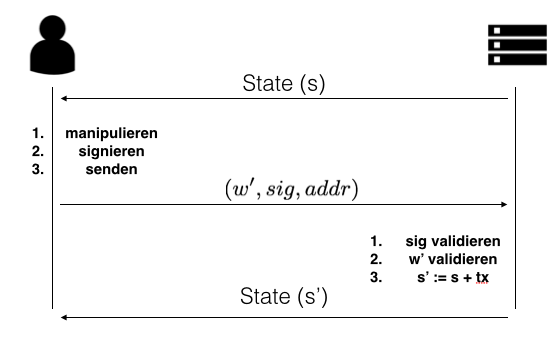
\includegraphics[width=1\textwidth]{bilder/interaktion.png}
  \caption{Interaktion eines Akteurs mit einer dao.}
  \label{intSeq}
\end{figure}

Der Akteur:
\begin{enumerate}
  \item Läd sich den für ihn relevanten Teil des Konsens herunter
  \item Manipuliert diesen, jedoch muss die Manipulation den Regeln der DAO folgen, da sie sonst von den Minern abgelehnt wird
  \item Signiert die Manipulation
  \item Sendet seine Transaktion an ihn bekannte Miner, damit diese zu einen Block hinzugefügt wird.
\end{enumerate}

Der Miner:
\begin{enumerate}
  \item Bekommt von unterschiedlichen Quellen Transaktionen
  \item Die Signatur jeder Transaktion wird validiert: ist der angegebene Akteur auch ihr Erzeuger?
  \item Die Manipulation des derzeitigen Zustandes wird validiert: ist die Manipulation des aktuellen Zustandes nach den aktuellen Regeln valide?
  \item Falls die Signatur und Manipulation valide ist, wird der derzeitige zustand aktualisiert und die Transaktion wird der Menge valider, bekannter Transaktionen hinzugefügt, die vom Miner in den nächsten Block hinzugefügt werden sollen.
  \item Der Miner versucht nun nach dem ``Proof of *'' Mechanismus eine Berechtigung vom Netzwerk zu erhalten um seinen privaten Konsens zum allgemeinen Konsens der DAO zu machen.
\end{enumerate}

Ein Akteur benötigt für das Agieren in der Ethereum DAO ein Bestand an der interner Währung. Wie viel, hängt von der Komplexität der ausgelösten Transaktion ab: Für jeden Berechnungsschritt wird ein kleiner Betrag erhoben. Ist nicht genügend Wert verfügbar, terminiert die Transaktion und wird vom Netzwerk abgelehnt. So wird auch das Halteproblem umgangen.

\begin{aquote}{Ethereum Whitepaper p. 28 \cite{Butterin2014}}
  [...] halting problem: there is no way to tell, in the general case, whether or not a given program will ever halt.
  [...] our solution works by requiring a transaction to set a maximum number of computational steps that it is allowed to take, and if execution takes longer computation is reverted but fees are still paid.
\end{aquote}

Eine Ethereum interne DAO besteht aus einem assoziativem Speicher der den Programmcode sowie Daten beinhaltet. Sie besitzt eine Adresse und hat einen Bestand an interner Währung: Ether.

Ein Beispiel für eine interne DAO ist eine dezentrale Währung, wie sie derzeit vom Bitcoin repräsentiert wird (Quelle \cite{Butterin2014}) ist in Abbildung \ref{contract1} illustriert, ein weiteres Beispiel in Abbildung \ref{contract2} ist ein dezentrales DNS System wie ihn die Namecoin DAO implementiert.

% ! Akteure = Programme | Benutzer


\begin{figure}[ht]
  \centering
\begin{lstlisting}
  from = msg.sender
  to = msg.data[0]
  value = msg.data[1]

  if self.storage[from] >= value:
  self.storage[from] = self.storage[from] - value
  self.storage[to] = self.storage[to] + value
\end{lstlisting}
  \caption{Nachbildung einer dezentralen Währung als Ethereum basierte DAO.}
  \label{contract1}
\end{figure}

\begin{figure}[ht]
  \centering
\begin{lstlisting}
  if !contract.storage[msg.data[0]]:
    contract.storage[msg.data[0]] = msg.data[1]
    return(1)
  else:
    return(0)
\end{lstlisting}
  \caption{Nachbildung eines dezentralen DNS als Ethereum basierte DAO.}
  \label{contract2}
\end{figure}

Diese beiden Beispiele illustrieren wie vergleichsweise einfach es ist eine DAO auf einer bestehenden Plattform, wie der von Ethereum, zu erstellen, anstadt der bisherigen Blockchain-Basierten Ansätzen. Ethereum gilt deshalb auch als DAO Platform welche die dezentralität der DAO von ihrer eigentlichen Funktionalität entkoppelt. Eine weitere wichtige Funktionalität einer DAO ist die der Wartbarkeit. Jedoch stellt sich hier die Frage nach dem Besitz und den Berechtigungen der Besitzer, die DAO manipulieren zu können. Hierfür muss ebenfalls ein Regelwerk gefunden werden, der die Wartung der DAO, im folgenden auch Selbst-Modifikation genannt, von ihrer eigentlichen Funktionalität entkoppelt. 


%%%%%%%%%%%%%%%%%%%%%%%%%%%%%%%%%%%%%%%%%%%%%%%%%%%%%%%%%%%%%%%%%
%%%%%%%%%%%%%%%%%%%%%%%%%%%%%%%%%%%%%%%%%%%%%%   GETEILTES OBJEKT
%%%%%%%%%%%%%%%%%%%%%%%%%%%%%%%%%%%%%%%%%%%%%%%%%%%%%%%%%%%%%%%%%

\chapter{Selbst-Modifikation-Schicht einer DAO}
\label{selfMod}
In diesem Kapitel wird die Selbst-Modifikation-Schicht einer DAO betrachtet. Hierfür wird in einer Einführung für die Notwendigkeit einer solchen Schicht argumentiert. In Kapitel \ref{smoddef} wird eine Definition einer solchen Schicht vorgeschlagen. In Kapitel \ref{smoddiskuss} werden die einzelnen Eigenschaften der Definition diskutiert. Für die Anwendung auf reguläre Grammatiken und die Implementation wird in Kapitel \ref{gramerw} eine Codierung durch eine Grammatikerweiterung vorgestellt. In Kapitel \ref{transsys} wird ein Transitionssystem für die Dynamik der Manipulation vorgestellt mit den dazugehörigen validen Transaktionen in Kapitel \ref{transvalid}.

Durch eine Plattform wie Ethereum wird nun das Erstellen von DAOs um ein vielfaches leichter gemacht, jedoch gibt es noch keine einheitliche Lösungsansätze um die DAOs oder generell dezentrale Inhalte ebenfalls auf eine dezentrale Weise zu erstellen oder diese zu modifizieren. Es Fehlt einer Entkopplung der DAO von den Regeln, wie diese von den Inhabern gerecht, also proportional zu ihrem Besitz, Manipuliert werden können.

% Derzeit - Linux/ Bitcoin/ Ethereum
Derzeit werden DAOs, entweder von einer einzelnen Schlüsselperson, einer Organisation (wie bei Bitcoin die ``Bitcoin-Foundation''\footnote{https://bitcoinfoundation.org/ 25.02.2015}) oder einem Unternehmen (wie bei Ethereum ``Ethereum Switzerland GmbH''\footnote{https://www.ethereum.org/ 25.02.2015}) entwickelt und manipuliert. Trotz der dezentralen Natur der DAOs ist die Kontrolle über diese noch Zentralisiert. 
% Die Zentralisierte Kontrolle ist eine notwendige Folge zweier Probleme:

Da es sich um Bitcoin und Ethereum um dezentrale Anwendungen handelt, ist es nicht trivial, wem diese Anwendungen gehören: Der Besitz lässt sich nicht determinieren. Falls man die interen Tokens aus der Blockchain Schicht ebenfalls als Besitzanteil an den DAOs interpretiert, so können die Besitzer nicht über die Manipulationen der Regeln der DAO mitentscheiden.

% Bitcoin - 100k ausschreibung
Das Problem ist in der Community jedoch bekannt. Im Juni 2014 hat Oliver Janssens, einer der Early-Adopter von Bitcoin ein Preisgeld von 100 000 USD in BTC an denjenigen ausgeschrieben, der ein Konzept vorschlägt, wie die Bitcoin Foundation auf dezentrale weise abgelöst werden kann.

\begin{aquote}{Reddit - Oliver Jansens http://redd.it/25sf4f 19.02.2015}
 The Bitcoin foundation [...] is internally recreating the same archaic political system that fails to work for society. Bitcoin is the currency of the internet generation. It puts the power back into the hands of the people. You cannot expect its main representative organisation to be exactly the opposite: A non-transparent, political and secretive elite.
\end{aquote}

Der Gewinner war die Bitcoin-Basierte dezentrale Crowdfunding Plattform Lighthouse\footnote{https://www.vinumeris.com/lighthouse}. Diese erfüllt nicht wirklich die Ansprüche an eine solche Selbst-Modifikation-Schicht.
% Problem - Benutzer/ Kandidaten werden echt groß
Der Mechanismus einer solchen Schicht muss einerseits eine große Anzahl an Stimmberechtigten Kandidaten (derzeit wurden rund 200k Bitcoin Adressen verwendet) berücksichtigen sowie eine ähnlich große Menge an Vorschlägen. Er sollte schnell und agil auf aufkommende Probleme reagieren können, jedoch niedrige Einstiegsbarrieren für Benutzer besitzen. Die Besitzverteilung sollte genau determiniert sein und die Manipulation der DAO gerecht - also proportional zu dem Besitz.

\textbf{Im folgenden möchte ich meinen Vorschlag einer solchen Schicht vorstellen. Hierfür werden wir als erstes die theoretischen Komponenten betrachten, dann ihre Anwendung auf die regulären Grammatiken und schließlich ihre Implementation.}


Theoretisch kann eine solcher Mechanismus durch ein \textbf{initialisiertes Transitionssysthem $T=(M,I,\tau)$} nach \cite{Glausch} modelliert werden. Hierzu muss eine passende Zustandsmenge definiert werden, einen Initialzustand sowie die Übergangsfunktion, die valide Manipulationen (Transitionen) der DAO beschreibt.

Durch die Dezentralisierung-Schicht wird sichergestellt, dass Transitionen \textbf{immer} von einem Akteur $a$ ausgelöst werden und das dieser Akteur ebenfalls ihr Urheber ist. Damit besitzen eine Transition die Form $(a, O')$. $O'$ beinhaltet dabei die Manipulationen des Akteurs.


\section{Definition}
\label{smoddef}
In der Selbst-Modifikation-Schicht können wir davon ausgehen, dass für die Dezentralität der DAO bereits gesorgt ist. Es handelt sich entweder selbst um eine Blockchain-Basierte DAO oder eine, die eine Plattform wie Ethereum benutzt. Insofern gilt die DEzentralität im folgenden als gegeben.

Eine DAO in einer Grammatik $G$ ist ein Tupel $O_G=(A, K, <, share, vote)$ bestehend aus:

\begin{enumerate}
\item eine endliche Menge von Akteuren $A$
\item eine eindeutige \textbf{Besitzverteilung} von Akteuren zur DAO
\begin{eqnarray}
  share: A \rightarrow \mathbb{N}
\end{eqnarray}
\item eine endliche Menge von validen \textbf{Kandidaten} mit mindestes einem Element 
\begin{eqnarray}
  K_G \subseteq L(G) \land |K_G| \geq 1
\end{eqnarray}
\item eine strickte Totalordnung der Kandidaten 
\begin{eqnarray}
   < \subset K\times K 
\end{eqnarray}
\item eine Bewertung der Kandidaten durch die Akteure. 
\begin{eqnarray}
  vote: A\times K \rightarrow [0,1]
\end{eqnarray}
\end{enumerate}

Sei $\mathbf{DAO_G} = \{ O_G\ |$ $O_G$ ist DAO in der einer Grammatik $G$ $\}$ die Menge aller DAOs in der Grammatik $G$.
% sowie $\mathbf{P_G}:= \{ K_G | K_G \subseteq L(G) \}$ die Menge aller möglichen Kandidatenmengen.

Zudem existiert eine Konsensfunktion die eine DAO in ein valides Wort überführt. 
\begin{eqnarray}
  consens: DAO_G \rightarrow L(G)
\end{eqnarray}


\section{Diskussion der Eigenschaften}
\label{smoddiskuss}

Im Folgenden werden die Eigenschaften eienr DAO nähr betrachtet: in \ref{kand} die Kandidaten, in \ref{besitz} die Besitzverteilung der Akteure zur DAO, in \ref{defkonsens} wird die einigung der Akterue auf einen Konsenskandidaten beschrieben, in \ref{daoex} wird ein anschauliches Beispiel einer DAO gegeben. Schließlich werden in \ref{quality} Qualitätskritärien für die Implementierung gegeben.

\subsection{Kandidaten}
\label{kand}
Der Hier verfolgte Ansatz ist nur DAOs in regulären Grammatiken zu Betrachten. Diese Eigenschaft schränkt die Menge der möglichen Kandidaten ein. Zu der Kandidatenmenge existiert eine strickte Ordnungsrelation, die die Reihenfolge angibt, in der die Kandidaten hinzugefügt wurde.

\subsection{Besitzverteilung}
\label{besitz}

%Aktienmodell

Die Besitzverteilung wird ähnlich dem Aktienmarkt Modelliert. Dabei hat eine DAO ein bestimmte Anzahl an Teilen (geschrieben $|O_G| \in \mathbb{N}$), die unter den Akteuren aufgeteilt sind. 

Die Funktion $share: A \rightarrow \mathbb{N}$ gibt den Anteil von $O_G$ an, der im Besitz von einem Akteur ist. 

\begin{eqnarray}
  |O_G| := \sum_{a \in A} share(a)
\end{eqnarray}

% Besitz = Bestimmung
Der Besitz einer DAO $O_G$ wird durch das Recht definiert, dieses Kontrollieren zu können\cite{Waldron2004}. Ist der Besitz unter mehreren Akteuren aufgeteilt, so gibt der Anteil am Objekt an, zu welcher Gewichtung jeder einzelne Akteur über die DAO mitbestimmen kann.

Eine Konsensfunktion entscheidet schließlich über die Ausführung der Kontrolle.

Für die Bestimmung der Besitzverteilung können einerseits die Tokens benutzt werden, die in der Dezentralisierung-Schicht verwendet werden. Andererseits können auch neue eingeführt werden. Für den Blockchain basierten Ansatz der Dezentralisierung muss bei getrennten Besitz-Tokens jedoch sicher gestellt werden, dass die Tokens der Blockchain-Schicht einen Wert für die Miner und damit eine motivierende Funktion am Mining-Prozess teilzunehmen besitzen. 

% Gilt $share_O(a) > 0$, so nennt man $a$ auch ein \textbf{Member} von $O$.
% 
% $M_O \subseteq A$ ist die Menge aller Member von $O$.




\subsection{Konsens}
\label{defkonsens}

\begin{eqnarray}
  consens: DAO_G \rightarrow L(G)
\end{eqnarray}

Die Konsensfunktion überführt jede DAO in ein Wort der $L(G)$ Sprache.
Dabei sucht die Funktion nach dem Kandidaten aus der Kandidatenmenge mit der maximalsten Bewertung. Die Bewertung eines Kandidaten ergibt sich dabei durch die Summe der gewichteten Bewertungen der Akteure. Falls mehrere Kandidaten die maximale Bewertung besitzen, wird der älteste Kandidat genommen.

\begin{eqnarray}
value(k) &:= \sum_{a\in A} share(a) \cdot vote(a,k)
consens (O_G) &:= min_<(\{ k |\ value(k) = \max_{k'\in K_G} (value(k')) \})
\end{eqnarray}


% \subsection*{Bewertung}

%todo: bewertung kann kontextfrei sein -> an die spracherweiterung binden? 
%todo: für kontextsensitive bewertungen gibt es 1) deligationen und 2) direkte kandidatenbewertungen

\subsection{Beispiel einer DAO}
\label{daoex}

Im folgenden ein Beispiel einer DAO $O_{G_{abc}}^1 := ( A, K, <, share, vote)$ für die Grammatik $G_{abc}$ definiert wie in \ref{regGramEx}.

\begin{eqnarray}
  A &=& HASH\\
  h_1 &=& 1HTN35UxBFTbcN8g2KfXC6TW2ipbytsysh\\
  h_2 &=& 16iF9qZWG1tKhnjnX5KKCYdYdLv4A1FQ4b\\
  h_3 &=& 1P3wGbbgDgLxivHw5BGGbLCHugsHBnjnjP\\
  share&:& hash\mapsto 
  \begin{cases}
    10 &: hash = h_1 \\
    7 &: hash = h_2 \\
    6 &: hash = h_3 \\
    0 &: otherwise
  \end{cases} \\
  K &=& \{aaaaa, aac, aacc, aaccc\} \\
  && aaaaa < aac < aacc < aaccc \\
  vote&:& hash,k\mapsto
  \begin{cases}
    1.0 &: hash = h_1, k = aaaaa \\
    0.9 &: hash = h_2, k = aacc \\
    0.9 &: hash = h_3, k = aacc \\
    0.9 &: hash = h_2, k = aaccc \\
    0.9 &: hash = h_3, k = aaccc \\
    0 &| otherwise \\
  \end{cases}
\end{eqnarray}
\label{daoExDef}

\begin{eqnarray}
consens(O_{G_{abc}}^1) &= aacc
\end{eqnarray}


\subsection{Qualitätskriterien}
\label{quality}

Für die Implementation ist auf folgende Qualitätskriterien zu achten:

\begin{description} 
  \item[\textbf{RESMIN:}]\hfill \\
    Es sind möglichst wenig Ressourcen (Speicher und Rechenleistung) vom Ethereum-Netzwerk notwendig, um Transaktionen zu validieren.
  \item[\textbf{INTMIN:}]\hfill \\
    Eine Akteur soll möglichst wenig Interaktionen benötigen, um auf eine gewünschte, von ihm erreichbare Manipulation zu kommen.
\end{description}

% 
%   * die Kandidatenmenge muss komprimiert werden, damit deren Speicherung möglichst wenig Speicher in anspruch nimmt.
%   * die validierung der manipulation muss eine kleine laufzeit haben.

% 

% es ist einfach für einen Akteur eine Bewertung über viele Kandidaten abzugeben.


%%%%%%%%%%%%%%%%%%%%%%%%%%%%%%%%%%%%%%%%%%%%%%%%%%%%%%%%%%%%%%%%%
%%%%%%%%%%%%%%%%%%%%%%%%%%%%%%%%%%%%%%%%%%%%%%     IMPLEMENTATION
%%%%%%%%%%%%%%%%%%%%%%%%%%%%%%%%%%%%%%%%%%%%%%%%%%%%%%%%%%%%%%%%%

\section{Grammatikerweiterung}
\label{gramerw}
Als Zustandsmenge für das Transitionssystem können wir nun die Menge aller möglichen DAOs nehmen. Allerdings muss man die Menge für die Implementation codieren sowie die Validitätsbedingungen auf der codierten Menge definieren. Eine passende Codierung die wir näher betrachten wollen ist eine DAO zu einem Wort einer Sprache zu machen. Diese Sprache nennen wir \textbf{Metasprache} der ursprünglichen Sprache ($L(G)$). Eine Bedingung muss jedoch sein, dass das Wort ohne Verlust von Informationen wieder zurück zur selben DAO decodiert werden kann. Damit können wir Transitionsbedingungen als Manipulationen des codierten Wortes definieren. 

Da die Wörter der codierten DAOs ebenfalls valide und invalide Teile der Wörter der ursprünglichen Sprache ($L(G)$) erkennen müssen und somit die Metasprache konstruierende Grammatik, ebenfalls die ursprüngliche Grammatik beinhalten muss, wird eine Funktion $S$ angegeben, die die ursprüngliche Grammatik $G$ so erweitert, dass diese zur gesuchten Metasprache wird $L(S(G))$.

Formaler gesagt muss eine Funktion $S: REG\rightarrow CFG$ gefunden werden, zusammen mit den Funktionen $\phi: DAO_G \rightarrow L(S(G))$ und $\phi^{-1}: L(S(G)) \rightarrow DAO_G$ für die die Eigenschaft $\phi\circ\phi^{-1} = id_{DAO_G}$ gilt.

Da die Funktion $S$, $\phi$ sowie $\phi^{-1}$ viele Komponenten haben, werden sie inkrementell eingeführt: Zuerst wird $S_1, \phi_1, \phi^{-1}_1$ definiert, diese codieren und decodieren die Kandidatenmenge einer DAO in ein Wort. Anschließend wird die Besitzverteilung sowie die Kandidatenbewertung ebenfalls eingearbeitet, sodass wir die gesuchten Funktionen erhalten.

\subsection{Codierung der Kandidatenmenge}
\label{codekand}
Die reguläre Grammatik wird so zu einer kontextfreien Grammatik erweitert, dass alle Wörter aus der Kandidatenmenge in einem Wort der erweiterten Grammatik codiert werden können. 

Dazu muss es eine Grammatik-Erweiterung $S_1: REG\rightarrow CFG$ gefunden werden.
Um zu zeigen, dass es sich bei $S_1$ um die gesuchte Erweiterung handelt, muss die Existenz der Funktionen $\phi_1: P(L(G)) \rightarrow L(S(G))$ und $\phi_1^{-1}: L(S(G)) \rightarrow P(L(G))$ gezeigt werden, für die die Bedingungen $\phi_1\circ\phi_1^{-1} = id_{P(L(G))}$ erfüllt ist.

Dieses kann mit Hilfe eine Trie-Datenstruktur realisiert werden, die redundant auftauchende Präfixe der Kandidaten zusammengefasst. Die Serialisierung der Tries ist eben ein Wort der Metasprache, die durch die Grammatikerweiterung $S_1$ konstruiert wird:

Sei $T(K_G)$ die Trie Datenstruktur, die die Menge $K_G$ codiert. Wir wissen, dass es eine Funktion $c: K_G \mapsto T(K_G)$ sowie $c^{-1}: T(K_G) \mapsto K_G$ existiert, für die $c\circ c^{-1} = id_{P(L(G))}$ gilt \cite{Morrison1968}. Zu finden ist demnach ein Isomorphismus $s: T(K_G) \mapsto w \in L(S_1(G))$ sowie $s^{-1}: w \in L(S_1(G)) \mapsto T(K_G)$ die ein Trie serialisieren und deserialisieren. Da ein Trie ein Baum ist wird für die Serialisierung einfach die geklammerte preorder Notation verwendet, die bekannterweise Isomorph ist. Damit haben wir die Funktionen $\phi_1 := c \circ s$ sowie $\phi_1^{-1} := c^{-1} \circ s^{-1}$ gefunden. 

Dieses wird anhand eines Beispiels für die Sprache $L(G) = \{ a^xb^yc^z\ |\ x,y,z\in \mathbb{N} \}$ und die Kandidatenmenge $\{aaaaa, aac, aacc, aaccc \}$ in Abbildung \ref{trieexk} durch die Trie $T(K_G)$ illustriert.

\begin{figure}[ht]
    \centering
    \Tree [.aa aaa c [.c c cc ] ]
    \caption{Trie für die Kandidatenmenge $\{aaaaa, aac, aacc, aaccc \}$}
    \label{trieexk}
\end{figure}

Mit der dazugehörigen preorder-Serialisierung die $[,]$ als Klammerzeichen sowie $\&$ als Trennzeichen verwendet:

\begin{eqnarray}
aa[aaa\&c\&c[c\&cc]]
\end{eqnarray}


Für die grammatik-erweiternde Funktion $S_1$ wird an jedem Ableitungsschritt in der Grammatik $G$ eine Mehrdeutigkeit zugelassen. Dafür werden die Produktionsregeln folgendermaßen erweitert:

\begin{eqnarray}
  P_{Options} := \{R \rightarrow [O_R], O_R \rightarrow r\& O_R, O_R \rightarrow r \ \vert\ R\rightarrow r\in P \land r\in \Sigma^*\} \\
\end{eqnarray}

Diese Mehrdeutigkeit ($[O_R]$) nennen wir \textbf{Optionsmenge} sowie die darin enthaltenen Elemente ($r$) \textbf{Option}. 

Eine solche Grammatikerweiterung erzeugt eben die Serialisierung einer Trie welche eine Menge valider Worte codiert:

\begin{eqnarray}
  aa[aaa\&c\&c[c\&cc]]\in L(S_1(G))
\end{eqnarray}

\subsubsection{Grammatik-Erweiterung S1}

Sei $G = (N,T,S,P)$ eine reguläre Grammatik.

$
\begin{array}{rl}
  S_1(G) :=& (N', T', S, P') \\
  N' :=& N \cup \{ O_R\ |\ (R\rightarrow r)\in P\land O_R \notin \Sigma\}\\
  T' :=& T \cup \{[ , ], \&\ |\ [,],\&\notin \Sigma \}\\
  P_{Options} :=& \{R \rightarrow [O_R], O_R \rightarrow r\& O_R, O_R \rightarrow r \ \vert\ R\rightarrow r\in P \land r\in \Sigma^*\} \\
  P' :=& P \cup P_{Options} 
\end{array}
$

% \subsection*{Definition $\phi$}
% 
% 
% 
% Sei $S(\alpha,K)$ die Funktion, die den Größten gemeinsamen Präfix aller Kandidaten liefert, die den Präfix $\alpha$ enthalten:
% 
% \[ E(\alpha, K) : \exists w\in K: w=\alpha\beta \] 
% 
% \[ 
%   A(\alpha, K): 
%     \exists ! \beta \forall x, y\in K\exists t, t' \in T\cup\{\varepsilon\}: \\
%     ( x = \alpha \beta t \gamma_1 \land y = \alpha \beta t' \gamma_2 ) \Rightarrow 
%     ( t = \gamma_1 = \varepsilon \lor t' = \gamma_2 = \varepsilon \lor t \neq t' )
% \] 
% 
% \[
%   S( \alpha, K ) := 
%   \begin{cases}
%     \beta & E(\alpha,K) \land A(\alpha,K) \\
%     \varepsilon & otherwise
%   \end{cases}
% \] 
%     
% % 1. Was ist wenn K leer ist, 
% %   s ist epsilon
% % was ist wenn K ein elementig ist, 
% %   
% % was ist wenn kein element den präfix alpha besitzt
% % was ist wenn alpha epsilon ist
% 
% Sei $U$ die Funktion, die einem Präfix und einer Kandidatenmenge die Wörter zuordnet, die nach diesem Präfix kommen.
% \[ U( \alpha, K ) := \{t S(\alpha t, K) |\ \alpha t \beta \in K \land ( t\in (T \lor t=\beta=\varepsilon )) \} \] 
% 
% Sei $Q$ die Funktion, die bei der übergabe einer Wortmenge K und einem präfix $\alpha$ eine Menge aller Wörter zurückliefert, die den Präfix $\alpha$ enthalten.
% 
% \[ Q(\alpha, K):= \{x |x\in K\land x=\alpha\beta\text{ mit } \beta \in T^*\} \] 
% 
% \[ 
%   O(\alpha, \beta, M):=
%   \begin{cases}
%     \beta & | |M| = 1 \\
%     \beta [E(\alpha, U( \alpha, M ), M)] &|otherwise
%     % [\bigcirc_{\beta \in U( \alpha, M )} (\beta O(\alpha \beta, Q(\alpha\beta, M))'\ ')] 
%   \end{cases}
% \] 
% 
% \[ 
%   E( \alpha, B, M ) := 
%   \begin{cases}
%     \varepsilon & |B =  \{ \varepsilon \}\\
%     \beta & |B =  \{ \beta \}\\
%     (O(\alpha, \beta, Q(\alpha\beta, M))'\ ' E(\alpha, B\setminus \{\beta\}, M))\text{ mit }\beta\in B &| otherwise
%   \end{cases}
% \] 
% 
% Dann ist $\phi := O( \varepsilon, S(\varepsilon, K), K)$ die gesuchte Funktion.
% 
% 
% \subsection*{Definition $\phi^{-1}$}
% 
% \[ 
%   \phi^{-1}(w) := 
%   \begin{cases}
%     U(\alpha, \beta) &| \alpha [ \beta ] = w \\
%     \{ w \}   &| otherwise
%   \end{cases}
% \] 
% 
% \[ 
%   U( \alpha, w ):= 
%   \begin{cases}
%     \phi^{-1}(\alpha x) \cup U(\alpha,s) &| w = x '\ ' s \\
%     \phi^{-1}(\alpha w) &|otherwise
%   \end{cases}
% \] 
% 
% \subsection*{zeige $\phi\circ\phi^{-1} = id_{P(K_G)}$}
% 
\TODO[inline]{ist hier ein formaler Beweis notwendig?}


\subsection{Codierung der Besitzverteilung}
Die Akteure lassen sich durch ein 20-Byte String genau identifizieren. Sei $HASH$ die Menge aller 20-Byte Strings. Im Folgenden werden die Hash-Strings in der Base58\footnote{https://en.bitcoin.it/wiki/Base58Check\_encoding 26.02.2015} Notation angegeben. Die Besitzverteilung ist eine Auflistung aller beteiligter Akteure sowie deren Anteile an der DAO.
Sei $hash\in HASH$ sowie $number\in\mathbb{N}$.

\begin{eqnarray}
P_{Acteurs} := \{A\rightarrow[hash\ number]A,A\rightarrow \varepsilon\}
\end{eqnarray}

Eine Beispiel-Verteilung ist: 

\begin{eqnarray}
  h_1 &=& 1HTN35UxBFTbcN8g2KfXC6TW2ipbytsysh\\
  h_2 &=& 16iF9qZWG1tKhnjnX5KKCYdYdLv4A1FQ4b\\
  h_3 &=& 1P3wGbbgDgLxivHw5BGGbLCHugsHBnjnjP\\
  a &=& [h_1\ 10][h_2\ 7][h_3\ 5] \\
  A &\rightarrow^*& a
\end{eqnarray}

In diesem Beispiel gehören Akteur $h_1$ - 10 Anteile, $h_2$ - 7 Anteile und $h_3$ - 5 Anteile. Somit ist die DAO - Größe 22 Anteile.

% \subsection{Optimierung der Kandidatenbewertung}

\subsection{Codierung der Kandidatenbewertung}
Um jede $DAO$ ohne Verlust von Information codieren zu können, muss jede mögliche Bewertungsverteilung von Akteuren und Kandidaten im Metawort enthalten sein können. 
Dieses kann erreicht werden, wenn die Bewertung der Kandidaten ($V$) an Optionen gebunden sind ($O_R \rightarrow r\& [V] O_R$). Da es für jeden Kandidaten aus der Kandidatenmenge genau eine Option gibt, die nur diesem Kandidaten zugeordnet ist (ein Blatt eines Tries), lässt sich jede Bewertungsverteilung des Kandidaten codieren, wenn sie dieser Option zugeordnet sind. Zusätzlich möchten wir Bewertungen einer Option zulassen, die mehreren Kandidaten zugeordnet sind. Dies sind solche, die wiederum eine Optionsmenge beinhalten. Wenn ein Akteur eine Option in einer Optionsmenge bewertet, so gibt er seine Stimme der Option im Kontext zu dem bisherigen Präfix des Wortes.
Die Bewertung dieser Option wird als ein Attribut in der Ableitung Synthetisiert\cite{Knuth1968} und damit jeweils von einer Bewertung einer tieferen Ebene ersetzt.

Sei $FLOAT = [0,1]$ die Menge der maschinell darstellbaren Fließkommazahlen zwischen 0 und 1: $float\in FLOAT$

\begin{eqnarray}
P_{Voting} := \{V\rightarrow [hash\ float]V, V \rightarrow \varepsilon\}
\end{eqnarray}
  
 Ein Beispiel ist:

\begin{eqnarray}
  h_1 &=& 1HTN35UxBFTbcN8g2KfXC6TW2ipbytsysh\\
  v &=& [h_1\ 1.0] \\
  V &\rightarrow^*& v \\
  O_R &\rightarrow^*& r\&[v]
\end{eqnarray}



\subsection{Codierung der Delegationen}

Für die Minimierung der Interaktion(INTMIN) wird transitives Abstimmen zugelassen. Akteure können nicht nur für die Option selbst abstimmen, sondern auch ihre Stimme für Optionsmengen an andere Akteure delegieren. Diese können im Kontext der delegierten Option für den Akteur mitbestimmen.

Ein solcher Akteur kann wiederum entweder eine Person, ein Zusammenschluss von Personen wie eine Interessengemeinschaft in Form einer DAO oder eine DAO ohne Fremdeinwirkung sein, die bestimmte Werte zu optimieren versucht.

Delegationen werden für Optionsmengen vererbt. Durch die lineare Struktur der Worte ergibt sich eine strickte Totalordnung der Delegationen, womit bei konkurierenden Delegationen immer die Delegation niedrigerer Ordnung genommen wird. Eine Stimme des Akteurs selbst, wird einer Stimme eines Deleganten vorgezogen.

\begin{eqnarray}
P_{Delegations} := \{D\rightarrow [hash\ hash]D,D\rightarrow [hash\ hash]\} 
\end{eqnarray}

Eine Beispiel-Verteilung ist: 

\begin{eqnarray}
  h_2 &=& 16iF9qZWG1tKhnjnX5KKCYdYdLv4A1FQ4b\\
  h_3 &=& 1P3wGbbgDgLxivHw5BGGbLCHugsHBnjnjP\\
  d &=& [h_2\ h_3] \\
  D &\rightarrow^*& d
\end{eqnarray}


% \TODO[inline]{roter faden}
% \subsection{Delegationsprogrammierung}
% Akteure können ihre Stimme nicht nur an externe Akteure delegieren, sondern auch an Contracts, welche in einer autonomen Weise abstimmen und so die Interessen der Akteure automatisch verfolgen. 
% 
% \subsection*{Beispiele}
% 
% Sei $G=(T,N,P,S)$ eine rechtsreguläre Grammatik mit:
% \[ T:=\{ a, b, c \}, N:=\{S\}, P:= \{S\rightarrow aS\ |\ bS\ |\ cS\ |\ \varepsilon \} \] 
% 
% Ein Delegationsprogramm kann mit dem Interesse entwickelt werden, nur für Kandidaten der kontextsensitiven Sprache $L = \{ a^nb^nc^n\ |\ n\in N\}$ zu stimmen so, dass falls die Mehrheit der Akteure ihm seine Stimme delegieren, der Konsens-Kandidat ebenfalls ein Element der Sprache $L$ sein wird. Auf diese weise lassen sich von den Akteuren komplexe Programme erstellen um die Kandidatenmenge agil und autonom zu bewerten.




\subsection{Vollständige Grammatik-Erweiterung S}
% \TODO[inline]{NUBER, HASH, FLOAT teil der Terminale}
% 
% \textbf{number} stellt eine ganzzahlige Nummer dar. \textbf{float}
% stellt eine Fließkommazahl dar, so dass $0\leq float \leq 1$. \textbf{hash} identifiziert einen Akteur, hier ist $hash$ ein 20 Bytes HEX-String. \\

\begin{align}
  S(G) :=& (N', T', S', P') \\
  N' :=& N \cup \{ O_R | (R\rightarrow r)\in P\land O_R \notin N\}\cup\{D, A, S'\}\\
  T' :=& T \cup \{[ , ], \&, |\ [,],\& \notin \Sigma \} \nonumber\\
  &\cup HASH
  \cup NUMBER
  \cup FLOAT 
  \\
  P_{Acteurs} :=& \{A\rightarrow[hash\ number]A,A\rightarrow \varepsilon \\
  &| hash\in HASH, number\in NUMBER\} \\
  P_{Options} :=& \{R \rightarrow [O_R][D], O_R \rightarrow r\& [V] O_R, O_R \rightarrow \varepsilon \ \nonumber\\
  &\vert\ R\rightarrow r\in P \land r\in \Sigma^*\} \\
  P_{Start} :=& \{S'\rightarrow [A][O_S][D]\} \\
  P_{Delegations} :=& \{D\rightarrow [hash\ hash]D,D\rightarrow [hash\ hash]\nonumber\\&| hash\in HASH\} \\
  P_{Voting} :=& \{V\rightarrow [hash\ float]V, V \rightarrow \varepsilon \nonumber \\&| hash\in HASH, float\in FLOAT\} \\
  P' :=& P
  \cup P_{Options} 
  \cup P_{Start} 
  \cup P_{Delegations} 
  \cup P_{Voting} 
  \cup P_{Acteurs}
\end{align}

\subsubsection*{Beispielwort}
Das zugehörige Metawort zur DAO $O_{G_{abc}}^1$ definiert wie in \ref{daoExDef} $\phi(O_{G_{abc}}^1) = w \in L(S(G))$ wird in der Abbildung \ref{metaword} dargestellt mit dem dazugehörige Konsens (\ref{examplekonsens}).

\begin{eqnarray}
consens(w) = aacc \label{examplekonsens}
\end{eqnarray}

\begin{figure}[ht]
  \centering
  \begin{lstlisting}
  [
    [h_1 10]
    [h_2 7]
    [h_3 5]
  ] [
    aa[
      aaa&[h_1 1.0]
      c&[]
      c[
        c&[]
        cc&[]
      ][]&[h_3 0.9]
    ][h_2 h_3]&[]
  ][]
  \end{lstlisting}
    \caption{Metawort $w\in L(S(G))$}
    \label{metaword}
\end{figure}





% \subsection*{zeige S(G) ist eindeutig}
% Leider gibt es kein Algorithmus, der beweist, dass S(G) eindeutig ist. Die eindeutigkeit ist jedoch ein notwendiges kritärium. Zumindest wurde die hier vorgestellte erweiterung für einige reguläre Grammatiken eindeutig von einem LALR(1) Parser akzeptiert wurde, was zumindest für diese eine eindeutigkeit zeigt. Wie man beweist, dass dieses für alle regulären gammatiken der Fall ist, muss noch gefunden werden.
% \TODO[inline]{AUF JEDEN FALL ÜBERARBEITEN - wie eindeutigkeit zeigen?}

\subsection{Konsens}

Nach dem die Kandidaten, die Akteure sowie ihre Anteile und die Bewertung der Kandidaten durch die Akteure in der Metasprache enthalten sind, erlaubt dies den Konsens der DAO als Interpretation des Wortes der $L(S(G))$ Sprache zu definieren. 

\begin{eqnarray}
consens: L(S(G)) \rightarrow L(G)
\end{eqnarray}

Die Idee hier ist, dass die transitive Hülle der Delegationen als
Attribut während der Ableitung vererbt(inherited) wird. Die Stimmenge 
wird hingegen als Attribut synthetisiert.\cite{Knuth1968} Delegationen zusammen mit den Stimmen quantifizieren jede Option aus einer Optionsmenge und wählen
eine Konsens-Option mit den Maximalsten Stimmen niedrigster Ordnung.


%%%%%%%%%%%%%%%%%%%%%%%%%%%%%%%%%%%%%%%%%%%%%%%%%%%%%%%%%%%%%%%%%
%%%%%%%%%%%%%%%%%%%%%%%%%%%%%%%%%%%%%%%%%%%%%%%%%    MANIPULATION 
%%%%%%%%%%%%%%%%%%%%%%%%%%%%%%%%%%%%%%%%%%%%%%%%%%%%%%%%%%%%%%%%%

\section{Transitionssystem}
\label{transsys}

Zur Wiederholung besteht ein Transitionssystem $T=(M,I,\tau)$ aus einer Zustandsmenge $M$, einem Initialzustand $I$ und einer Übergangsfunktion $\tau$.
Nach dem wir nun die Zustandsmenge als Metasprache $M=L(S(G))$ sowie die Codierung und Decodierung einer DAO in ein Wort der Metasprache gefunden haben, widmen wir uns der Übergangsfunktion $\tau$.

Als Initialzustand wird ein beliebiges Wort aus der Metasprache verwendet, welches weder Stimmen, noch Delegationen beinhaltet.

\begin{eqnarray}
I = \{s_0\in L(S(G))\}
\end{eqnarray}

Wir werden uns auf die Manipulation der Kandidatenmenge sowie der Kandidatenbewertung beschränken. Weitere Manipulationen werden in Aussicht gestellt. Valide Manipulationen der Kandidatenmenge soll das Erstellen und das Erweitern von Optionsmengen sein. Für die Kandidatenbewertung sollen das Hinzufügen und Entfernen der eigenen Stimmen sowie der eigenen Delegationen für Optionsmengen valide sein. 

Falls die Besitzverteilung von der Blockchain-Schickt übernommen wird, greift die Dynamik dieser Schickt ebenfalls auf den derzeitigen Zustand des Metawortes. Wir möchten uns jedoch auf solche DAOs beschränken, bei denen die Besitzverteilung ausschließlich in der Selbst-Modifikation-Schicht manipuliert wird. Hier möchten wir das Überweisen eines Akteurs von eigenen Anteilen an einen anderen Akteur zulassen.


% 
% \subsection*{Zustände}
% 
% Sei $G = (N,T,S,P)$ eine rechtsreguläre Grammatik sowie
% $S(G)=(N',T',S',P')$ die dazugehörige erweiterte Grammatik.
% 
% Ein Zustand ist eine Struktur der Form $(L(S(G)), w) \in M$
% 
% % U ist die Trägermenge der Struktur und besteht aus den Wörtern der Sprache $L(S(G))$:
% % \[U := L(S(G))\]
% 
% % $consens$ ist die für $L(S(G))$ definierte konsens Funktion:
% $w\in L(S(G))$ ist das derzeitige Wort

\subsection{Aktualisierung}
Durch die Blockchain-Schicht ist jede Interaktion mit einer DAO eindeutig und nachweislich einem Akteur zugeordnet. Demnach ist jede Aktualisierung des derzeitigen Zustandes $w := s_i$ ein Tupel $\delta = (a,w')$ mit $hash=a\in A=HASH,\ w'\in L(S(G))$.

Sei $\Delta \subseteq A\times L(S(G))$ die Menge aller vom Miner gesehenen Aktualisierungen, die noch nicht auf Validität überprüft wurden und somit nicht Teil seines privaten Konsenses sind.


Akteure können jederzeit die Aktualisierungsmenge erweitern in dem sie eine Aktualisierung an einen Miner schicken: 
\begin{eqnarray}
\Delta' := \Delta \cup \{(a,w')\}
\end{eqnarray}


\subsection{Transformation}
Sei $\Delta \neq \emptyset$ 

\begin{eqnarray}
  \tau( w ) = 
  \begin{cases}
    w'  &: \exists (a,w') \in \Delta \land \beta(a,w,w') = true \\
    w   &: andernfalls 
  \end{cases}
\end{eqnarray}

Nach jeder Transformation wird die Aktualisierungsmenge ebenfalls aktualisiert, in dem die für die Transformation verwendete Aktualisierung entfernt wird. Wurde keine Aktualisierung verwendet, so sind alle Aktualisierungen invalide:

\begin{eqnarray}
  \Delta' = 
  \begin{cases}
    \Delta\setminus \{ (a, w' )\} &: (a,w')\text{ wurde in der Transformation verwendet} \\
    \{\} &: andernfalls
  \end{cases}
\end{eqnarray}


\section{Validierung der Aktualisierung}
\label{transvalid}

Um die Validität einer Transformation zu testen, wird das derzeitige Wort $w$ zusammen mit dem auslösenden Akteur $a$ sowie seinem manipuliertem Wort $w'$ betrachtet. Die Transformation ist valide, falls die Kandidatenmenge wie in Abschnitt \ref{manipulationkandidaten} vorgestellt manipuliert wird, die Kandidatenbewertung wie in Abschnitt \ref{manipulationbewertung} vorgestellt manipuliert wird oder die Anteile wie in Abschnitt \ref{manipulationanteile} vorgestellt manipuliert werden.

% \subsection*{ACID Eigenschaft der Transaktionen}
% 
% Atomicity - Daten-Operationen entweder ganz oder gar nicht ausgeführt wird
% 
% Consistency - Sequenz von Daten-Operationen nach Beendigung einen konsistenten Datenzustand hinterlässt
% 
% Isolation - nebenläufig in Ausführung befindliche Daten-Operationen gegenseitig beeinflussen
% 
% Durability - erfolgreichen Abschluss einer Transaktion garantiert dauerhaft in der Datenbank gespeichert sind




\subsection{Manipulation der Kandidaten}
\label{manipulationkandidaten}
Eine Optionsmenge kann an jeder Position im Wort erzeugt oder erweitert werden, solange das neu vorgeschlagene Wort, ein Wort der Metasprache ist, sowie die Bewertungen der Kandidaten nicht verändert werden.
\begin{eqnarray}
(A,K',share',vote') = \phi^{-1}(w') \nonumber\\
\land (A,K,share,vote) = \phi^{-1}(w) \nonumber\\
\Rightarrow vote = vote' \\
  w'\in L(S(G))
\end{eqnarray}
Die neu hinzukommenden Optionen dürfen keine Delegationen oder Stimmen enthalten, sowie noch nicht in der bisherigen Optionsmenge enthalten sein.

\subsubsection{Erzeugen einer Optionsmenge}

Sei $S(G) = (T', N', S', P')$ eine erweiterte Grammatik. Sei weiter $O,S'\in N'$ sowie $v,o_1,o_2 \in T'^*$, $o_1\neq 0_2$ und $0\leq i\leq j\leq n$ mit $i,j,k,n \in \mathbb{N}$

\begin{eqnarray}
  w &=& w_{0 .. i-1}\ w_{i..j}\ w_{j+1 .. n} \\
  w_{i..j} &=& \alpha o_1 \& [v] \\
  O &\rightarrow^*& \alpha R \& [v] \\
  R &\rightarrow^*& o_1 \\
  S' &\rightarrow^*& w_{0 .. (i-1)}\ O\ w_{(j+1) .. n}\\
  R &\rightarrow^*& o_2 \\
  w' &=& w_{0..i-1}\ \alpha [o_1\& [v] o_2\& []][]\ w_{j+1 .. n}
\end{eqnarray}


Für $w$ hat $O$ folgende Struktur:
\begin{center}
\Tree [.O $\alpha$ [.R $o_1$ ] $\&$ $\lbrack$ [.V v ] $\rbrack$ [.O ... ] ]
\end{center}


Für $w'$ besitzt O folgende Struktur:
\begin{center}
\Tree [.O $\alpha$ [.R $\lbrack$ [.O $o_1$ $\&$ $\lbrack$ [.V v ]  $\rbrack$ [.O $o_2$ $\&$ $\lbrack$ [.V $\epsilon$ ] $\rbrack$ ] ] $\rbrack$ $\lbrack$ [.D $\epsilon$ ] $\rbrack$ ] $\&$ $\lbrack$ $\rbrack$ [.O ... ] ]
\end{center}

Dabei muss $o_2$ frei von Delegationen und Stimmen sein.

\TODO[inline]{ist hier ein Beweis das die Kritärien nicht verletzt werden notwendig?}

\subsubsection{Erweitern einer Optionsmenge}
 
Sei $o,d,r \in T'^*$ sowie $R,O_R \in N'$

\begin{eqnarray}
  w &=& w_{0 .. i-1}\ w_{i..j}\ w_{j+1 .. n} \\
  w_{i..j} &=& \alpha[o][d] \\
  R   & \rightarrow ^*& w_{i..j}\\
  O_R & \rightarrow_P^*& o\\
  O_R & \rightarrow ^* & r\\
  w' & = & w_{0..(i-1)}\ \alpha[o r\& []][d]\ w_{(j+1)..n} 
\end{eqnarray}

$r$ muss dabei Delegations- und Stimmfrei sein sowie neu:
\begin{eqnarray}
(A,K',share',vote') = \phi^{-1}(w_{0..i-1}\ \alpha[r\& []][d]\ w_{j+1..n}) \\\land (A,K,share,vote) = \phi^{-1}(w) \\\Rightarrow K'\cap K = \emptyset
\end{eqnarray}


\subsection{Manipulation der Kandidatenbewertung}
\label{manipulationbewertung}

Sei für alle Manipulationen $a\in HASH$ der auslösende Akteur.

\subsubsection{Hinzufügen einer Stimme}
Sei $b_1,b_2,v,r \in T'^*$

\begin{eqnarray}
  w &=& w_{0 .. i-1}\ w_{i..j}\ w_{j+1 .. n} \\
  v &\neq& b_1 a b_2 \\
  w_{i..j} &=& r\& [v] \\
  w' &=& w_{0 .. i-1}\ r \& [v[a\ n]]\ w_{j+1 .. n}
\end{eqnarray}

\subsubsection{Löschen einer Stimme}

Sei $v_1, v_2 \in T'^*$ sowie $n\in\mathbb{N}$

\begin{eqnarray}
  w &=& w_{0 .. i-1}\ w_{i..j}\ w_{j+1 .. n} \\
  w_{i..j}&=& r\& [v_1 [a\ n] v_2] \\
  w' &=& w_{0..(i-1)} r\& [v_1\ v_2] w_{(j+1)..n}
\end{eqnarray}


\subsubsection{Hinzufügen einer Delegation}
Da die Reihenfolge der Delegationen wichtig ist, für die Auflösung konkurierender Delegationen, daher ist das Hinzufügen einer Delegation an jeder Stelle in einer Delegationsmenge möglich.

Sei $o,d_i \in T'^*$ sowie $h'\in HASH$ und $h\neq a$

\begin{eqnarray}
  w &=& w_{0 .. i-1}\ w_{i..j}\ w_{j+1 .. n} \\
  u,v &\in& \{ w | w = ([h_1\ h_2])^*\text{ mit } h_1,h_2 \in HASH \} \\
  w_{i..j} &=& [o][uv] \\
  w' &=& w_{0 .. (i-1)}\ [o][u[a\ h']v]\ w_{(j+1) .. n}
\end{eqnarray}

\subsubsection*{Löschen einer Delegation}

Sei $o,d_i \in T'^*$ sowie $h'\in HASH$

\begin{eqnarray}
  w &=& w_{0 .. i-1}\ w_{i..j}\ w_{j+1 .. n} \\
  u,v &\in& \{ w | w = ([h_1\ h_2])^*\text{ mit } h_1,h_2 \in HASH \} \\
  w_{i..j} &=& [o][u[a\ h']v] \\
  w' &=& w_{0 .. (i-1)}\ [o][uv]\ w_{(j+1) .. n}
\end{eqnarray}

\subsection{Überweisung von Anteilen}
\label{manipulationanteile}

Ein Akteur kann seine Anteile an einen Anderen überweisen. Dabei müssen die Fälle unterschieden werden, ob der Empfänger bereits Anteile hält, bei dem Fall wird die Überweisungssumme seinen Beständen addiert, oder ob es sich um einen neuen Akteur handelt. Dieser wird mit der Überweisungssumme neu hinzugefügt. 

Sei $h'\in HASH$ mit $h' \neq a$ sowie $l,m,n\in\mathbb{N}$
\TODO[inline]{hier ist zum ersten mal nicht die Symbolkonkatination gemeint sondern die Interpretation der werte(+,-), muss das als Interpretation geschrieben werden?}

\begin{eqnarray}
  w &=& w_{0 .. i-1}\ w_{i..j}\ w_{j+1 .. n} \\
  b_1, b_2, b_3, b_4, b_5, b_6 &\in& \{ w | w = ([h\ n])^*\text{ mit } h \in HASH\text{ und }n\in\mathbb{N} \} \\
  w_{i..j} &=& [ b_1 b_2 b_3 [a\ n] b_4 b_5 b_6 ] \\
  m' &=& (m+l) \\
  n' &=& (n-l) \\
  n - l &\geq& 0\\
  \text{Fall 1: } &&b_2 = [h' m]\\
  w' &=& w_{0 .. (i-1)}\ [ b_1 [h' m'] b_3 [a\ n'] b_4 b_5 b_6 ]\ w_{(j+1) .. n} \\
  \text{Fall 2: } &&b_5 = [h' m]\\
  w' &=& w_{0 .. (i-1)}\ [ b_1 b_2 b_3 [a\ n'] b_4 [h' m'] b_6 ]\ w_{(j+1) .. n}\\
  \text{Fall 3: } && \\
  w' &=& w_{0 .. (i-1)}\ [ b_1 b_2 b_3 [a\ n'] b_4 b_5 b_6 [h' l]]\ w_{(j+1) .. n}
\end{eqnarray}



\chapter{Implementation}
\label{implementation}

In diesem Kapitel wird die Implementation der Anwendung einer Selbst-Modifikations-Schicht auf DAOs regulärer Grammatik vorgestellt. Dafür wird in Kapitel \ref{architecture} die gewählte Architektur vorgestellt sowie in Kapitel \ref{metalang} der Umgang mit Grammatiken und der Metasprache.

Implementiert wurde im Rahmen dieser Arbeit eine \textbf{zentralisierte} Version der Selbst-Modifikation-Schicht. Die Dezentralität wurde erst einmal ignoriert, da die Funktionsweise der Selbst-Modifikation im Vordergrund steht. Jedoch sind alle Grundlagen dafür gelegt die hier erarbeitete Lösung auf Ethereum oder eine andere Turing-Vollständige DAO Platform zu portieren und damit zu dezentralisieren.


\section{Architektur}
\label{architecture}

\begin{figure}[ht]
    \centering
    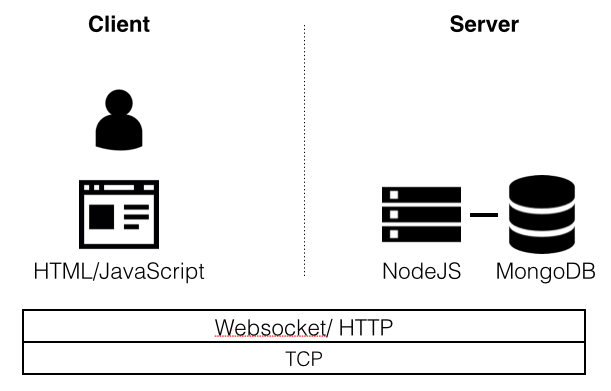
\includegraphics[width=1\textwidth]{bilder/client-server.png}
    \caption{Benutzte Technologie}
    \label{client-server}
\end{figure}

Ziel der Implementation ist einerseits eine lauffähige Implementierung des Konzeptes. Andererseits einem Benutzer zu ermöglichen mit Anwendungsbeispielen zu experimentieren: reguläre Grammatiken anzulegen sowie diese mit der Angabe der Besitzverteilung und eines Initialwortes zu einer DAO zu machen.
Implementiert ist die Interaktion mit der DAO Selbst-Modifikation-Schicht wie in \ref{interaction} beschrieben. Ein Akteur kann dabei entweder eine vorhandene DAO manipulieren oder eine neue erstellen. Technisch wurde hier eine Klassische Client-Server Architektur benutzt wie sie in Abbildung \ref{client-server} illustriert ist. Dafür wurde das MeteorJS\footnote{http://meteor.com 25.02.2015} Web Framework verwendet
welches auf NodeJS\footnote{http://nodejs.org/ 25.02.2015} basiert - einem serverseitigen JavaScript Compiler. Für die Datenspeicherung wird MongoDB\footnote{http://www.mongodb.org/ 25.02.2015} verwendet - eine NoSQL Datenbank. Der Client kommuniziert über HTTP und WebSocket mit dem Server.

%http://yuml.me/diagram/scruffy/class/draw
%2F%2F Cool Class Diagram, 
% [DAO| name:String; parentID: ForeignKey; state: Number; actor:String; word:String; sig: String ]-          parentID>[DAO| name: String; parentID: ForeignKey; state: Number; actor: String; word: String; sig: String],
% [DAOName| name: String; remoteID: ForeignKey; grammarID: ForeignKey] -> [DAO],
% [DAOName] -> [Grammar| name: String; bnf: JSON; extended: JSON ]

\begin{figure}[ht]
    \centering
    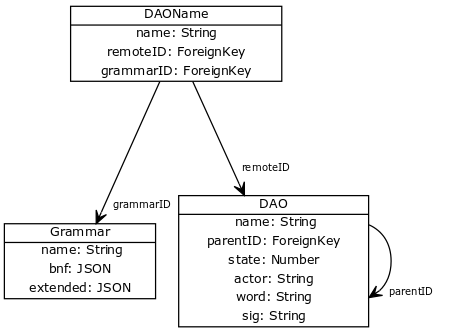
\includegraphics[width=0.60\textwidth]{bilder/dataModel.png}
    \label{datamodel}
    \caption{Datenmodell}
\end{figure}

Das Datenmodell(Abbildung \ref{datamodel}) ist in zwei Bereiche unterteilt: Einerseits die DAOs und andererseits die Grammatiken. 

Ein Akteur hat nun die Möglichkeiten 

\begin{enumerate}
  \item Vorhandene Grammatiken aufzulisten
  \item Eine vorhandene Grammatik zu inspizieren
  \item Eine neue Grammatiken hinzuzufügen
  \item DAOs aufzulisten
  \item Den Aufbaue und die Historie einer DAO einzusehen
  \item Eine DAO zu manipulieren
  \item Eine neue DAO zu erstellen
\end{enumerate}

Für die Signierung wird die Bibliothek BitcoinJS-lib\footnote{https://github.com/bitcoinjs/bitcoinjs-lib 26.02.2015} verwendet. Sie stellt die notwendigen ECDSA sowie SHA Funktionen zu Verfügung. Für dem Umgang mit Grammatiken und Worten wird JISON\footnote{http://zaach.github.io/jison 26.02.2015} eine JavaScript Portierung des Bison/Flex LALR(1) Parser-Generators verwendet.
%   LALR(1) 
%     Subset of CFG
%     S(G) is in LALR(1)

BitcoinJS-lib stellt notwendige kryptografische Funktionen bereit: das Erstellen von einem Private-Key auf Basis eines Strings, das erstellen eines Public-Key und einer Adresse auf Basis des Private-Keys, das Signieren von Nachrichten mit einem Private-Key sowie das Verifizieren von Nachrichten mit ihrer Signatur und einer Adresse. Dieses deckt alle Funktionen ab, die für die sichere Kommunikation von einem Akteur und der DAO notwendig sind.

\section{Metasprache}
\label{metalang}
\begin{figure}[ht]
    \centering
    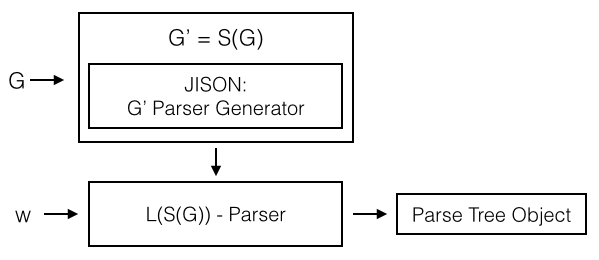
\includegraphics[width=0.90\textwidth]{bilder/parsergenerator.png}
    \caption{Grammatikerweiterung und Parser Generator}
\end{figure}

Für das erzeugen von Parsern wird der Parser-Generator JISON so erweitert, dass dieser bei Eingabe einer regulären Grammatik $G$ einen Parser für die zur Grammatik zugehörigen Metasprache erzeugt. Dieser Parser interpretiert eine Wort der $L(S(G))$ Sprache als ein Parse Baum Objekt (PTO). Eine Grammatik wird als Bison Grammatik (Abbildung \ref{bisongrammar}) in der EBNF Schreibweise angegeben.

\begin{figure}[ht]
  \centering
  \begin{lstlisting}
  %lex
  %%
  \s                           /* IGNORE */
  (a)                          return 'a'
  (b)                          return 'b'
  (c)                          return 'c'
  .                            return 'INVALID'
  /lex

  %start A
  %% 


  A: 'a' A | 'a'
   | 'b' B | 'b'
   | 'c' C | 'c'
   | ;

  B: 'b' B | 'b'
   | 'c' C | 'c';

  C: 'c' C | 'c';
  %%
  \end{lstlisting}
  \caption{ Bison Grammatik für die Sprache $L(G) = \{ a^xb^yc^z | x,y,z\in \mathbb{N} \}$ }
  \label{bisongrammar}
\end{figure}

Das Parse Baum Objekt besitzt folgende Funktionen:

\paragraph*{toString}
wandelt das Parse Baum Objekt wieder um in ein Wort der Metasprache, das dieses Parse Baum Objekt konstruiert.

\paragraph*{getConsensString}
wählt den Konsens-Kandidaten aus:
wendet die Konsensfunktion an und liefert ein Wort der $L(G)$ Sprache zurück.
% der Kandidat mit der maximalsten Bewertung sowie der 

\paragraph*{validate}
erhält ein weiteres (PTO), die eine Manipulation des derzeitigen PTOs beinhaltet, sowie eine Akteur-Adresse und überprüft ob die Manipulation des derzeitigen PTOs vom Akteur valide ist.

\paragraph*{add}
erhält ein Wort $w$ der $L(G)$ Sprache und fügt es dem Derzeitigen PTO hinzu. Diese Operation fügt der DAO einen neuen Kandidaten hinzu.

\paragraph*{getCandidates}
liefert $K_G$ der DAO zurück: ein Array aller Kandidaten mit ihren Bewertungen. Dadurch lässt sich leicht die Funktion $vote$ rekonstruieren.


% \subsection*{ abc - Grammatik }
% \subsection*{ reddit - Grammatik }
% \subsection*{ memGenerator - Grammatik }


% section  (end)

%%%%%%%%%%%%%%%%%%%%%%%%%%%%%%%%%%%%%%%%%%%%%%%%%%%%%%%%%%%%%%%%%
%%%%%%%%%%%%%%%%%%%%%%%%%%%%%%%%%%%%%%%%      IMPLEMENTATIONSPLAN
%%%%%%%%%%%%%%%%%%%%%%%%%%%%%%%%%%%%%%%%%%%%%%%%%%%%%%%%%%%%%%%%%
% \section{Umfang der Arbeit}
% 
% \subsection*{Implementation}
% \begin{itemize}
%   \item Eine Zentralisierte Version der $L(S(G))$-Sprache sowie des Transitionssystem wird implementiert.
%   \begin{itemize}
%     \item JISON\footnote{http://jison.org/}, eine javascript Portierung des Bison\footnote{http://www.gnu.org/software/bison/}/Flex\footnote{http://flex.sourceforge.net/} LALR(1) Parser Generators wird so erweitert, dass bei Eingabe einer beliebigen regulären Grammatik $G$ im bison Format\footnote{http://dinosaur.compilertools.net/bison/bison\_6.html} dieser einen Parser erzeugt welcher Wörter aus der $L(S(G))$ Sprache als Eingabe bekommt und ein öffentliches Transitionssystem erzeugt.
%     \item Ein Initialisierungs-Script, welches aus einem Wort der $L(G)$ Sprache und einer Besitzverteilung gegeben als $\{(a,n)| a\in\ 20byteHexString \land n\in \mathbb{N} \}$ ein valides initiales Wort in der $L(S(G))$ Sprache erzeugt.
%     \item Akteure können durch eine Webseite in die Transaktionshistorie einsehen, sowie das Wort valide manipulieren.
%     \item Eine Client-seitige asymmetrische Verschlüsselung validiert die Transaktionen der Akteure.
%     \item Die Konsens-Funktion wird ebenfalls Implementiert und erzeugt zu jedem Stand einen öffentlich verfügbaren Konsens-Kandidaten.
%   \end{itemize}
%   \item Einige anschauliche Beispiele regulärer Sprachen mit beispielhaften Delegationsprogrammen werden implementiert und demonstriert.
% \end{itemize}




% \listoftodos[Aufgaben]



%%%%%%%%%%%%%%%%%%%%%%%%%%%%%%%%%%%%%%%%%%%%%%%%%%%%%%%%%%%%%%%%%
%%%%%%%%%%%%%%%%%%%%%%%%%%%%%%%%%%%%%%%%%%%%%%%%%%       Aussicht
%%%%%%%%%%%%%%%%%%%%%%%%%%%%%%%%%%%%%%%%%%%%%%%%%%%%%%%%%%%%%%%%%

\chapter{Zusammenfassung und Ausblick}
\label{ausblick}
% outline nochmal
% Auswertung - bewertende zusammenfassung


\section{Anwendung auf kontextfreie Grammatiken}

Eine interessante Anwendung des hier vorgestellten Ansatzes einer Selbst-Modifikation-Schicht ist die Anwendung auf die kontextfreien Sprachen. Damit können alle Programmiersprachen zumindest Syntaktisch abgebildet werden. Dieses ist jedoch nicht Trivial. Das Problem hierbei ist die Kodierung der Kandidatenmenge. Auf Grund der Limitierung der Ableitungsregeln kann ein Ableitungsbaum einer regulären Grammatik keine Knoten haben, die mehrere Kinder mit Nichtterminalen Besitzen(Äste). Somit ist der Ableitungsbaum eine lineare Struktur. Dieses ermöglicht die Konstruktion eines Präfixbaumes bei dem Äste als Optionen angesehen werden. 
Zwar lässt sich die Zusammenfassung der Kandidaten bei kontextfreien Grammatiken mit der selben Methode anhand des Ableitungsbaumes konstruieren, jedoch multiplizieren sich die Optionen in unterschiedlichen Kindern eines Knotens. Dadurch gilt die in \ref{codekand} geforderte Bedingung $\phi_1\circ\phi_1^{-1} = id_{P(L(G))}$ nicht, da Optionen hinzu kommen. Ebenfalls lässt sich nicht jede Kandidatenbewertung durch das Anhängen an Optionsknoten codieren.

Betrachten wir einmal das Beispiel der Sprache $L(G) = { [ab][abc] }$ mit der konstruierenden Grammatik: 

\begin{eqnarray}
  G &=& (T,N,P,S)\\
  T &=& \{ a, b \}\\
  N &=& \{ S, B \} \\
  P &=& \{ S\rightarrow BB, B\rightarrow a, B\rightarrow b\}
\end{eqnarray}

Die Kandidatenmenge $K_1={ab, ac, ba}$
Sowie das anhand des Ableitungbaumes valide Metawort: 

\[ [A][ a\&[v_1]b\&[v_2] ][][ a\&[v_3]b\&[v_4]c\&[v_5] ][] ][] \] 


Die sich aus dem Metawort bildenden Kandidaten sind: $K_2=\{ aa, bb, ab, ba, ac, bc \}$

Weiter gibt es kein Mechanismus der jedes mögliche Kandidatenbewertung in der Sprache darstellen kann: Es stehen in diesem Beispiel 5 Bewertungsvariablen für 6 Kandidaten zur Verfügung. 

\section{Dezentralisierung}
Wie bereits erwähnt ist die Dezentralisierung der Selbst-Modifikation-Schicht der DAO z.B. durch eine Portierung auf die Ethereum Plattform der nächste notwendige Schritt.

\section{Anonymisierung}
Durch die Pseudonyme Natur der Anteilseigener lassen sich Rückschlüsse darüber ziehen, welcher Akteur für welche Option abgestimmt hat. Dadurch lässt sich der Konsens manipulieren in dem auf strategisch wichtige Akteure Druck ausgeübt wird um ihre Stimme zu ändern. Auch wird das Abstimmverhalten der Anteilseigener beeinflusst, da diese fürchten könnten ihre Pseudonymen Status verlieren zu können. Die Anonyme Wahl ist ebenfalls ein Kriterium für demokratische Wahlen in vielen Organisationen, sodass eine Anonymisierung der Abstimmung eine weitere erstrebenswerte Erweiterung ist. Diese Anonymisierung könnte durch Homomorphe Verschlüsselung\cite{Gentry2009} oder durch andere kryptografische Mittel realisiert werden. Siehe dazu \cite{Fouard}.

\section{Manipulation der Besitzverteilung}
Derzeit ist die Größe einer DAO fest, sodass die einzige Möglichkeit an Anteile zu gelangen, diese von Anderen überwiesen zu bekommen ist. Eine mögliche Erweiterung währe die der Erschaffung neuer Anteile. Diese können entweder von der DAO verkauft oder anhand festgelegter Regeln herausgegeben werden. Ein Beispiel Regelsatz währe das binden an Optionsmengen. Derjenige Akteur erhält die neuen Anteile, dessen vorgeschlagene Option für eine bestimmte Dauer den Platz der Konsens-Option einnimmt.

% \subsection*{Manipulation der Grammatik}
% Ein weiterer, jedoch Spekulativer Schritt währe die manipulation der grammatik


%%%%%%%%%%%%%%%%%%%%%%%%%%%%%%%%%%%%%%%%%%%%%%%%%%%%%%%%%%%%%%%%%
%%%%%%%%%%%%%%%%%%%%%%%%%%%%%%%%%%%%%%%%%%%%%%%%%%%%      QUELLEN
%%%%%%%%%%%%%%%%%%%%%%%%%%%%%%%%%%%%%%%%%%%%%%%%%%%%%%%%%%%%%%%%%


\newpage

\nocite{Otto}
\nocite{Vasant2015}
\bibliography{library}

\bibliographystyle{alpha}

\end{document}
